\documentclass[]{article}
\usepackage{lmodern}
\usepackage{amssymb,amsmath}
\usepackage{ifxetex,ifluatex}
\usepackage{fixltx2e} % provides \textsubscript
\ifnum 0\ifxetex 1\fi\ifluatex 1\fi=0 % if pdftex
  \usepackage[T1]{fontenc}
  \usepackage[utf8]{inputenc}
\else % if luatex or xelatex
  \ifxetex
    \usepackage{mathspec}
  \else
    \usepackage{fontspec}
  \fi
  \defaultfontfeatures{Ligatures=TeX,Scale=MatchLowercase}
  \newcommand{\euro}{€}
\fi
% use upquote if available, for straight quotes in verbatim environments
\IfFileExists{upquote.sty}{\usepackage{upquote}}{}
% use microtype if available
\IfFileExists{microtype.sty}{%
\usepackage{microtype}
\UseMicrotypeSet[protrusion]{basicmath} % disable protrusion for tt fonts
}{}
\usepackage[margin=1in]{geometry}
\usepackage{hyperref}
\PassOptionsToPackage{usenames,dvipsnames}{color} % color is loaded by hyperref
\hypersetup{unicode=true,
            pdftitle={ggplotFL: plotting FLR objects with ggplot2},
            pdfborder={0 0 0},
            breaklinks=true}
\urlstyle{same}  % don't use monospace font for urls
\usepackage{color}
\usepackage{fancyvrb}
\newcommand{\VerbBar}{|}
\newcommand{\VERB}{\Verb[commandchars=\\\{\}]}
\DefineVerbatimEnvironment{Highlighting}{Verbatim}{commandchars=\\\{\}}
% Add ',fontsize=\small' for more characters per line
\usepackage{framed}
\definecolor{shadecolor}{RGB}{248,248,248}
\newenvironment{Shaded}{\begin{snugshade}}{\end{snugshade}}
\newcommand{\KeywordTok}[1]{\textcolor[rgb]{0.13,0.29,0.53}{\textbf{{#1}}}}
\newcommand{\DataTypeTok}[1]{\textcolor[rgb]{0.13,0.29,0.53}{{#1}}}
\newcommand{\DecValTok}[1]{\textcolor[rgb]{0.00,0.00,0.81}{{#1}}}
\newcommand{\BaseNTok}[1]{\textcolor[rgb]{0.00,0.00,0.81}{{#1}}}
\newcommand{\FloatTok}[1]{\textcolor[rgb]{0.00,0.00,0.81}{{#1}}}
\newcommand{\ConstantTok}[1]{\textcolor[rgb]{0.00,0.00,0.00}{{#1}}}
\newcommand{\CharTok}[1]{\textcolor[rgb]{0.31,0.60,0.02}{{#1}}}
\newcommand{\SpecialCharTok}[1]{\textcolor[rgb]{0.00,0.00,0.00}{{#1}}}
\newcommand{\StringTok}[1]{\textcolor[rgb]{0.31,0.60,0.02}{{#1}}}
\newcommand{\VerbatimStringTok}[1]{\textcolor[rgb]{0.31,0.60,0.02}{{#1}}}
\newcommand{\SpecialStringTok}[1]{\textcolor[rgb]{0.31,0.60,0.02}{{#1}}}
\newcommand{\ImportTok}[1]{{#1}}
\newcommand{\CommentTok}[1]{\textcolor[rgb]{0.56,0.35,0.01}{\textit{{#1}}}}
\newcommand{\DocumentationTok}[1]{\textcolor[rgb]{0.56,0.35,0.01}{\textbf{\textit{{#1}}}}}
\newcommand{\AnnotationTok}[1]{\textcolor[rgb]{0.56,0.35,0.01}{\textbf{\textit{{#1}}}}}
\newcommand{\CommentVarTok}[1]{\textcolor[rgb]{0.56,0.35,0.01}{\textbf{\textit{{#1}}}}}
\newcommand{\OtherTok}[1]{\textcolor[rgb]{0.56,0.35,0.01}{{#1}}}
\newcommand{\FunctionTok}[1]{\textcolor[rgb]{0.00,0.00,0.00}{{#1}}}
\newcommand{\VariableTok}[1]{\textcolor[rgb]{0.00,0.00,0.00}{{#1}}}
\newcommand{\ControlFlowTok}[1]{\textcolor[rgb]{0.13,0.29,0.53}{\textbf{{#1}}}}
\newcommand{\OperatorTok}[1]{\textcolor[rgb]{0.81,0.36,0.00}{\textbf{{#1}}}}
\newcommand{\BuiltInTok}[1]{{#1}}
\newcommand{\ExtensionTok}[1]{{#1}}
\newcommand{\PreprocessorTok}[1]{\textcolor[rgb]{0.56,0.35,0.01}{\textit{{#1}}}}
\newcommand{\AttributeTok}[1]{\textcolor[rgb]{0.77,0.63,0.00}{{#1}}}
\newcommand{\RegionMarkerTok}[1]{{#1}}
\newcommand{\InformationTok}[1]{\textcolor[rgb]{0.56,0.35,0.01}{\textbf{\textit{{#1}}}}}
\newcommand{\WarningTok}[1]{\textcolor[rgb]{0.56,0.35,0.01}{\textbf{\textit{{#1}}}}}
\newcommand{\AlertTok}[1]{\textcolor[rgb]{0.94,0.16,0.16}{{#1}}}
\newcommand{\ErrorTok}[1]{\textcolor[rgb]{0.64,0.00,0.00}{\textbf{{#1}}}}
\newcommand{\NormalTok}[1]{{#1}}
\usepackage{longtable,booktabs}
\usepackage{graphicx,grffile}
\makeatletter
\def\maxwidth{\ifdim\Gin@nat@width>\linewidth\linewidth\else\Gin@nat@width\fi}
\def\maxheight{\ifdim\Gin@nat@height>\textheight\textheight\else\Gin@nat@height\fi}
\makeatother
% Scale images if necessary, so that they will not overflow the page
% margins by default, and it is still possible to overwrite the defaults
% using explicit options in \includegraphics[width, height, ...]{}
\setkeys{Gin}{width=\maxwidth,height=\maxheight,keepaspectratio}
\setlength{\parindent}{0pt}
\setlength{\parskip}{6pt plus 2pt minus 1pt}
\setlength{\emergencystretch}{3em}  % prevent overfull lines
\providecommand{\tightlist}{%
  \setlength{\itemsep}{0pt}\setlength{\parskip}{0pt}}
\setcounter{secnumdepth}{0}

%%% Use protect on footnotes to avoid problems with footnotes in titles
\let\rmarkdownfootnote\footnote%
\def\footnote{\protect\rmarkdownfootnote}

%%% Change title format to be more compact
\usepackage{titling}

% Create subtitle command for use in maketitle
\newcommand{\subtitle}[1]{
  \posttitle{
    \begin{center}\large#1\end{center}
    }
}

\setlength{\droptitle}{-2em}

  \title{ggplotFL: plotting FLR objects with ggplot2}
    \pretitle{\vspace{\droptitle}\centering\huge}
  \posttitle{\par}
    \author{}
    \preauthor{}\postauthor{}
      \predate{\centering\large\emph}
  \postdate{\par}
    \date{03 October, 2018}


% Redefines (sub)paragraphs to behave more like sections
\ifx\paragraph\undefined\else
\let\oldparagraph\paragraph
\renewcommand{\paragraph}[1]{\oldparagraph{#1}\mbox{}}
\fi
\ifx\subparagraph\undefined\else
\let\oldsubparagraph\subparagraph
\renewcommand{\subparagraph}[1]{\oldsubparagraph{#1}\mbox{}}
\fi

\usepackage{underscore}

\begin{document}
\maketitle

The R package \texttt{ggplot2} offers a plotting style and tools that
are increasingly becoming a data visualization standard. One of the
added values of \texttt{ggplot2} is the ease in displaying highly
dimensional data in an intuitive way. For these reasons there are a
number of standard methods implemented in the package \texttt{ggplotFL}
to plot FLR objects, stock assessment diagnostics and MSE results. In
addition, standard \texttt{ggplot2} methods and functions can be used by
converting FLR objects into data frames, thus giving an extra
flexibility in plotting.

\section{Required packages}\label{required-packages}

To follow this tutorial you should have installed the following
packages:

\begin{itemize}
\tightlist
\item
  CRAN:
  \href{https://cran.r-project.org/web/packages/ggplot2/index.html}{ggplot2}
\item
  FLR: \href{http://www.flr-project.org/FLCore/}{FLCore},
  \href{http://www.flr-project.org/ggplotFL/}{ggplotFL}
\end{itemize}

You can do so as follows,

\begin{Shaded}
\begin{Highlighting}[]
\KeywordTok{install.packages}\NormalTok{(}\StringTok{"ggplot2"}\NormalTok{)}
\KeywordTok{install.packages}\NormalTok{(}\KeywordTok{c}\NormalTok{(}\StringTok{"ggplotFL"}\NormalTok{), }\DataTypeTok{repos=}\StringTok{"http://flr-project.org/R"}\NormalTok{)}
\end{Highlighting}
\end{Shaded}

\begin{Shaded}
\begin{Highlighting}[]
\CommentTok{# Load all necessary packages, trim pkg messages}
\KeywordTok{library}\NormalTok{(FLCore)}
\KeywordTok{library}\NormalTok{(ggplotFL)}

\CommentTok{# Load datasets for tutorial}
\KeywordTok{data}\NormalTok{(}\StringTok{"ple4"}\NormalTok{)}
\KeywordTok{data}\NormalTok{(}\StringTok{"ple4sex"}\NormalTok{)}
\KeywordTok{data}\NormalTok{(}\StringTok{"nsher"}\NormalTok{)}
\end{Highlighting}
\end{Shaded}

\section{\texorpdfstring{Using \texttt{ggplot2} with \emph{FLR}
objects}{Using ggplot2 with FLR objects}}\label{using-ggplot2-with-flr-objects}

The \texttt{ggplot2} package provides a powerful alternative paradigm
for creating both simple and complex plots in R using the ideas of
Wilkinson's \emph{Grammar of Graphics}.

To facilitate the use of \texttt{ggplot2} methods in \emph{FLR}, the
\texttt{ggplotFL} package has been created. The main resources on offer
in this package are overloaded versions of the \texttt{ggplot()} method
that directly accept certain \emph{FLR} classes, a new set of basic
plots for some \emph{FLR} classes based on \texttt{ggplot2} instead of
\texttt{lattice}, and some examples and documentation on how best to
make use of \texttt{ggplot2}'s powerful paradigm and implementation to
obtain high quality plots for even fairly complex data structures.

\subsection{\texorpdfstring{The overloaded \texttt{ggplot}
method}{The overloaded ggplot method}}\label{the-overloaded-ggplot-method}

The standard \texttt{ggplot} function expects a \texttt{data.frame} for
its first argument, \emph{data}. If \texttt{ggplot} is called with an
\emph{FLR} object, a conversion to \texttt{data.frame} takes place, and
any other arguments provided get passed to the original
\texttt{ggplot()}. The conversion makes use of
\texttt{as.data.frame}\footnote{\texttt{method?as.data.frame(\textquotesingle{}FLQuant\textquotesingle{})}}
methods defined in \texttt{FLCore}, with the \emph{cohort} argument set
to \emph{TRUE}.

As an example, the \texttt{FLStock} of \texttt{ple4} is a list
containing a number of elements.

\begin{Shaded}
\begin{Highlighting}[]
\CommentTok{# summary of the FLStock}
\KeywordTok{summary}\NormalTok{(ple4)}
\end{Highlighting}
\end{Shaded}

\begin{verbatim}
An object of class "FLStock"

Name: PLE 
Description: Plaice in IV. ICES WGNSSK 2018. FLAAP 
Quant: age 
Dims:  age  year    unit    season  area    iter
    10  61  1   1   1   1   

Range:  min max pgroup  minyear maxyear minfbar maxfbar 
    1   10  10  1957    2017    2   6   

catch         : [ 1 61 1 1 1 1 ], units =  t 
catch.n       : [ 10 61 1 1 1 1 ], units =  1000 
catch.wt      : [ 10 61 1 1 1 1 ], units =  kg 
discards      : [ 1 61 1 1 1 1 ], units =  t 
discards.n    : [ 10 61 1 1 1 1 ], units =  1000 
discards.wt   : [ 10 61 1 1 1 1 ], units =  kg 
landings      : [ 1 61 1 1 1 1 ], units =  t 
landings.n    : [ 10 61 1 1 1 1 ], units =  1000 
landings.wt   : [ 10 61 1 1 1 1 ], units =  kg 
stock         : [ 1 61 1 1 1 1 ], units =  t 
stock.n       : [ 10 61 1 1 1 1 ], units =  1000 
stock.wt      : [ 10 61 1 1 1 1 ], units =  kg 
m             : [ 10 61 1 1 1 1 ], units =  m 
mat           : [ 10 61 1 1 1 1 ], units =   
harvest       : [ 10 61 1 1 1 1 ], units =  f 
harvest.spwn  : [ 10 61 1 1 1 1 ], units =   
m.spwn        : [ 10 61 1 1 1 1 ], units =   
\end{verbatim}

By calling \texttt{as.data.frame()} on an \texttt{FLStock}, the list is
collapsed to a dataframe that than can be plotted by selecting the right
dimensions in terms of slot, age, iter, etc.. :

\begin{Shaded}
\begin{Highlighting}[]
\KeywordTok{head}\NormalTok{(}\KeywordTok{as.data.frame}\NormalTok{(ple4))}
\end{Highlighting}
\end{Shaded}

\begin{longtable}[c]{@{}llrllllr@{}}
\toprule
slot & age & year & unit & season & area & iter & data\tabularnewline
\midrule
\endhead
catch & all & 1957 & unique & all & unique & 1 & 78360\tabularnewline
catch & all & 1958 & unique & all & unique & 1 & 88785\tabularnewline
catch & all & 1959 & unique & all & unique & 1 & 105186\tabularnewline
catch & all & 1960 & unique & all & unique & 1 & 117975\tabularnewline
catch & all & 1961 & unique & all & unique & 1 & 119541\tabularnewline
catch & all & 1962 & unique & all & unique & 1 & 126290\tabularnewline
\bottomrule
\end{longtable}

\subsection{\texorpdfstring{\texttt{FLQuant}}{FLQuant}}\label{flquant}

Passing an \texttt{FLQuant} object to ggplot, we can specify the names
of the dimensions as variables in the plot, where \texttt{data} refers
to the column storing the actual numeric values. For example, to plot
\emph{data} (the \emph{catch} slot from \texttt{ple4} in this case)
against year, we could use

\begin{Shaded}
\begin{Highlighting}[]
\KeywordTok{ggplot}\NormalTok{(}\DataTypeTok{data =} \KeywordTok{catch}\NormalTok{(ple4), }\KeywordTok{aes}\NormalTok{(year, data)) +}\StringTok{ }\KeywordTok{geom_point}\NormalTok{() +}\StringTok{ }\KeywordTok{geom_line}\NormalTok{() +}\StringTok{ }\KeywordTok{ylab}\NormalTok{(}\StringTok{"Catch (t)"}\NormalTok{) +}\StringTok{ }\KeywordTok{xlab}\NormalTok{(}\StringTok{"Year"}\NormalTok{)}
\end{Highlighting}
\end{Shaded}

\begin{center}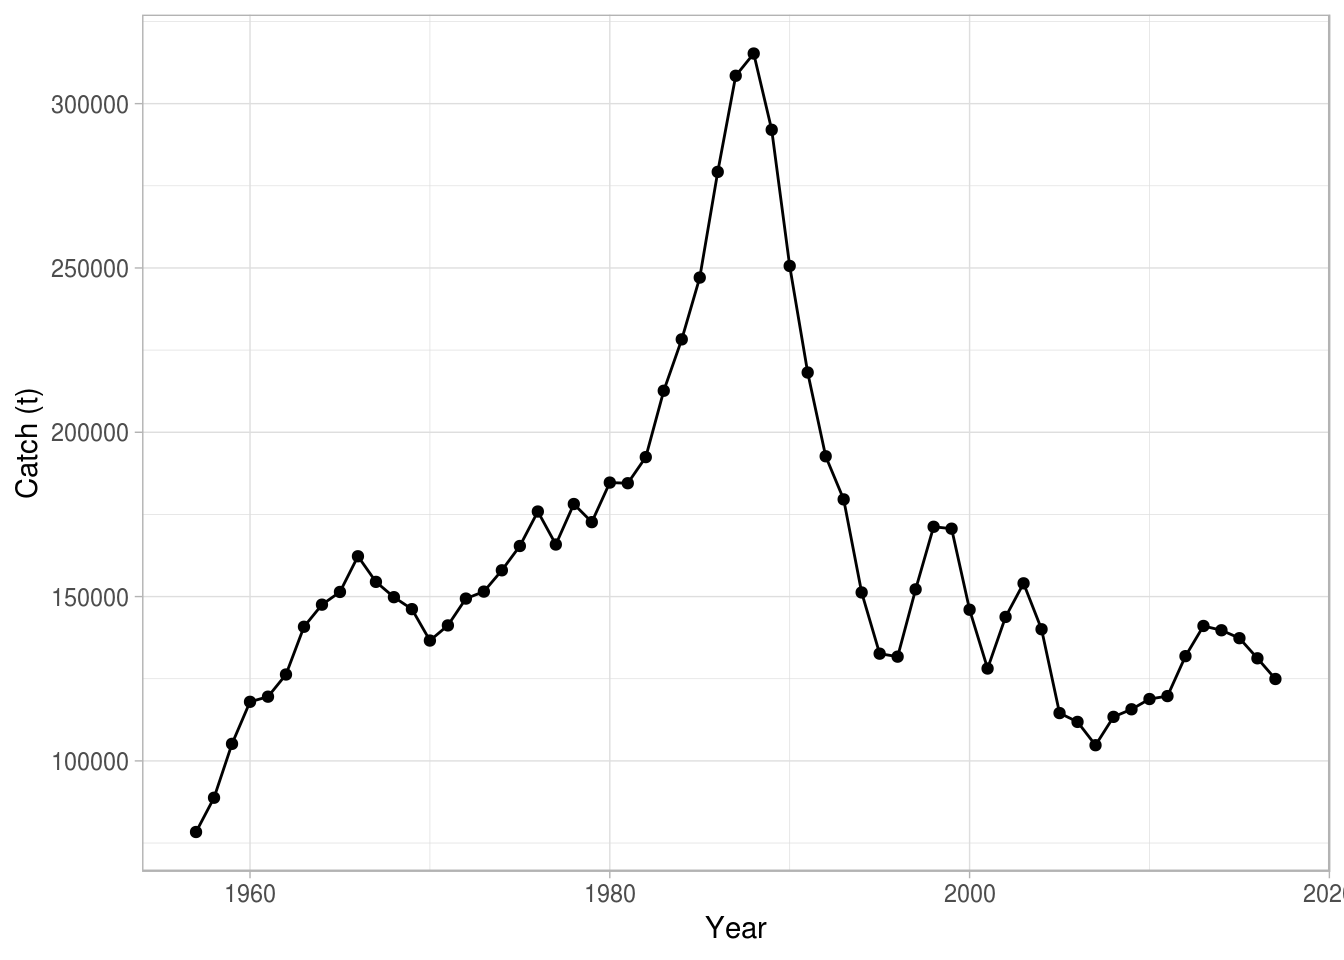
\includegraphics{docs/pdf/ggplotFL_plotting_FLR_objects_with_ggplot2_files/figure-latex/plotflquant-1} \end{center}

where we pass directly an \texttt{FLQuant} object for the \emph{data}
argument in \texttt{ggplot}, specify an aesthetic mapping
(\texttt{aes(year,\ data)}), and add both points
(\texttt{geom\_point()}) and lines (\texttt{geom\_line()}), together
with the appropriate axis labels.

\subsection{\texorpdfstring{\texttt{FLQuants}}{FLQuants}}\label{flquants}

Similarly, we can pass on to \texttt{ggplot} an object of class
\texttt{FLQuants}, and the conversion to \texttt{data.frame} will make
use of the corresponding method \footnote{\texttt{method?as.data.frame(\textquotesingle{}FLQuants\textquotesingle{})}}.
A new column gives the name of each \texttt{FLQuant} in the list, called
\emph{qname}. We can then use it to, for example, define a call to
\texttt{facet\_wrap()} to obtain a separate subplot per element.

\begin{Shaded}
\begin{Highlighting}[]
\KeywordTok{ggplot}\NormalTok{(}\DataTypeTok{data=}\KeywordTok{FLQuants}\NormalTok{(}\DataTypeTok{Yield=}\KeywordTok{catch}\NormalTok{(ple4), }\DataTypeTok{SSB=}\KeywordTok{ssb}\NormalTok{(ple4), }\DataTypeTok{F=}\KeywordTok{fbar}\NormalTok{(ple4)), }\KeywordTok{aes}\NormalTok{(year, data)) +}\StringTok{ }
\StringTok{  }\KeywordTok{geom_line}\NormalTok{() +}\StringTok{ }\KeywordTok{facet_wrap}\NormalTok{(~qname, }\DataTypeTok{scales=}\StringTok{"free_y"}\NormalTok{, }\DataTypeTok{nrow=}\DecValTok{3}\NormalTok{) +}\StringTok{ }\KeywordTok{labs}\NormalTok{(}\DataTypeTok{x=}\StringTok{""}\NormalTok{, }\DataTypeTok{y=}\StringTok{""}\NormalTok{)}
\end{Highlighting}
\end{Shaded}

\begin{figure}

{\centering 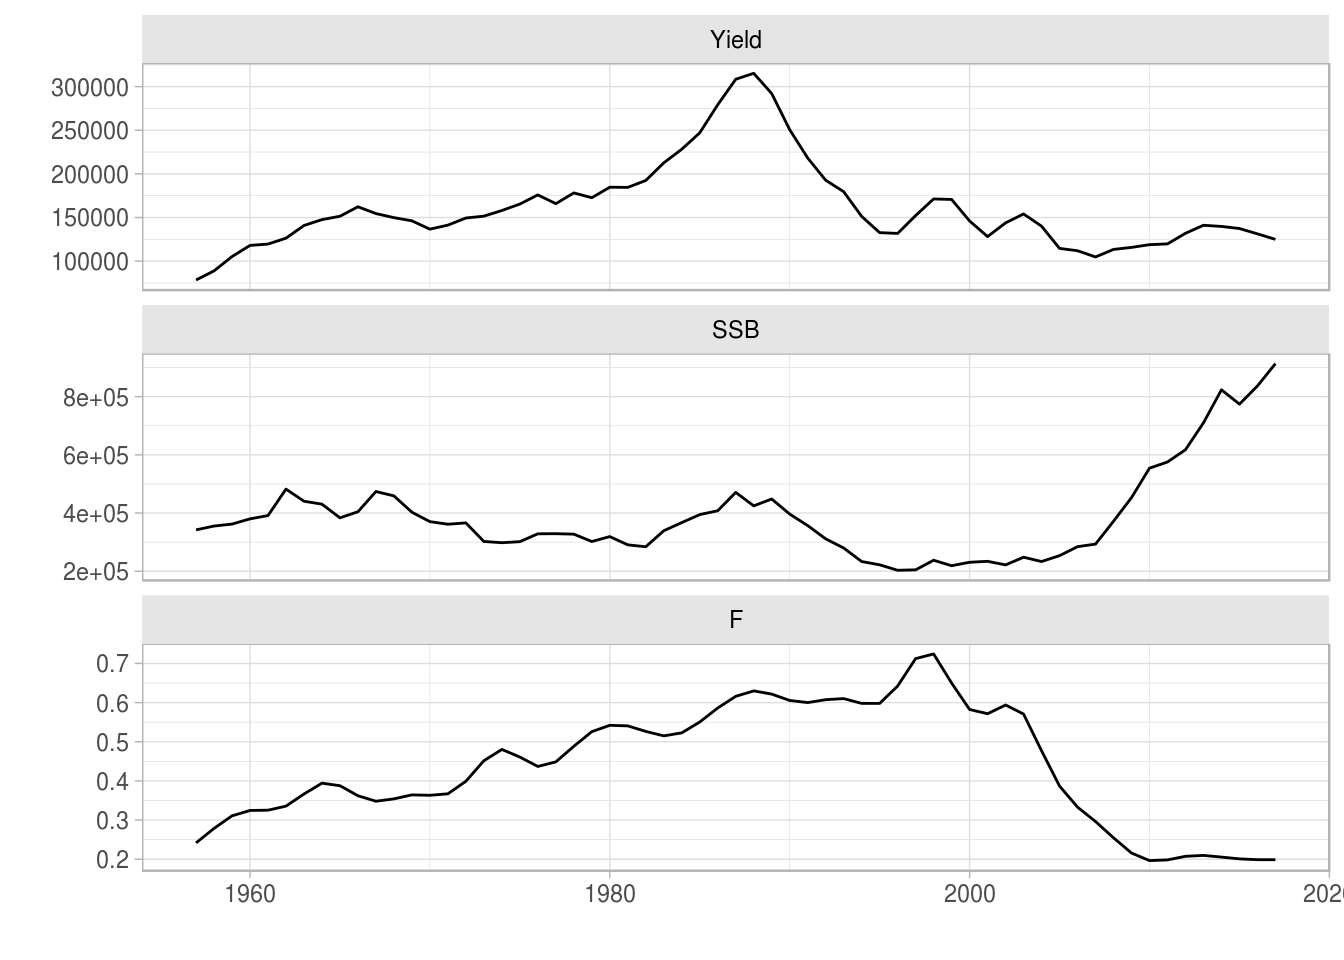
\includegraphics{docs/pdf/ggplotFL_plotting_FLR_objects_with_ggplot2_files/figure-latex/ggflqs-1} 

}

\caption{Facet wrap line plot of time series from an FLQuants object.}\label{fig:ggflqs}
\end{figure}

This procedure is particularly useful when plotting information from
objects with multiple \texttt{FLQuant} slots, because a subset of slots
can be selected for plotting. Furthermore, transformations or
computations can even be carried out in the call to the
\texttt{FLQuants()} creator.

\subsection{\texorpdfstring{\texttt{FLStock}}{FLStock}}\label{flstock}

A whole \texttt{FLStock} object can also be used as argument to
\texttt{ggplot()}, even if the heterogeneity in scale of the data
contained makes the plot slightly confusing. For example, we can plot
time-series of every \texttt{FLQuant} slot in \texttt{ple4}, with colour
applied to different age dimensions, by calling

\begin{Shaded}
\begin{Highlighting}[]
\KeywordTok{ggplot}\NormalTok{(}\DataTypeTok{data=}\NormalTok{ple4, }\KeywordTok{aes}\NormalTok{(year, data)) +}\StringTok{ }\KeywordTok{geom_line}\NormalTok{(}\KeywordTok{aes}\NormalTok{(}\DataTypeTok{group=}\NormalTok{age, }\DataTypeTok{colour=}\KeywordTok{factor}\NormalTok{(age))) +}\StringTok{ }
\StringTok{  }\KeywordTok{facet_wrap}\NormalTok{(~slot, }\DataTypeTok{scales=}\StringTok{"free"}\NormalTok{, }\DataTypeTok{nrow=}\DecValTok{3}\NormalTok{) +}\StringTok{ }\KeywordTok{labs}\NormalTok{(}\DataTypeTok{x=}\StringTok{""}\NormalTok{, }\DataTypeTok{y=}\StringTok{""}\NormalTok{) +}\StringTok{ }\KeywordTok{theme}\NormalTok{(}\DataTypeTok{legend.position =} \StringTok{"none"}\NormalTok{)}
\end{Highlighting}
\end{Shaded}

\begin{figure}

{\centering 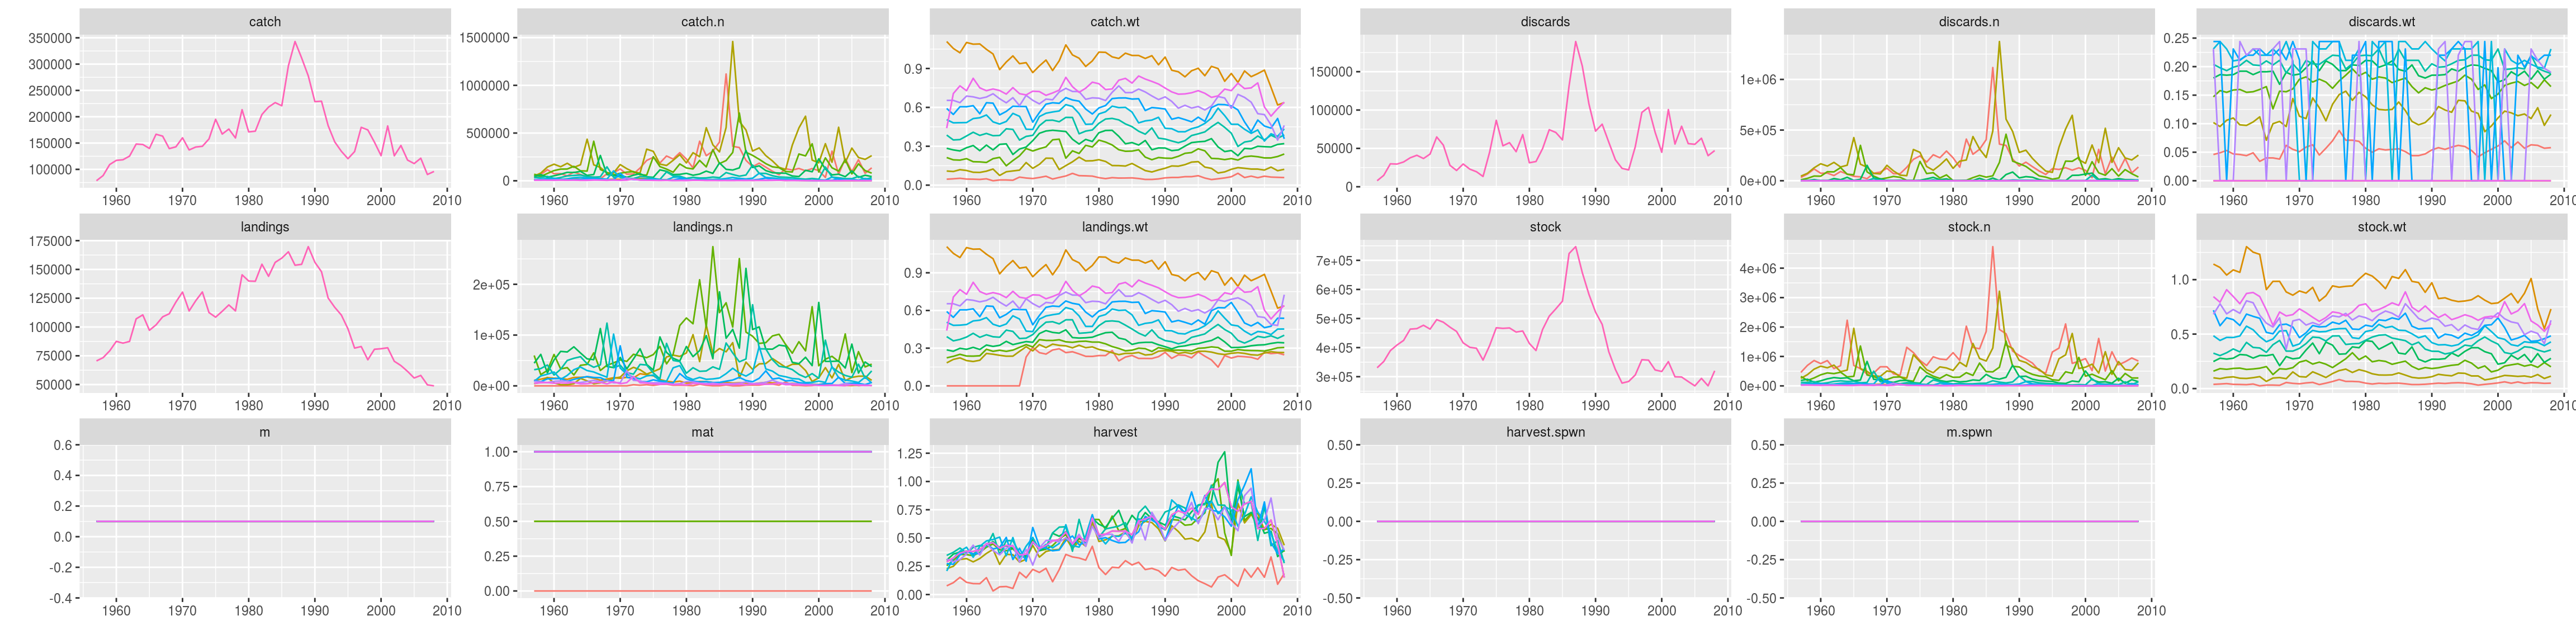
\includegraphics{docs/pdf/ggplotFL_plotting_FLR_objects_with_ggplot2_files/figure-latex/ggfls-1} 

}

\caption{Overall `ggplot` of an `FLStock` object, faceted by slot.}\label{fig:ggfls}
\end{figure}

\section{\texorpdfstring{New \texttt{plot()} methods for FLR
classes}{New plot() methods for FLR classes}}\label{new-plot-methods-for-flr-classes}

The \texttt{ggplotFL} package also provides new versions of the
\texttt{plot} method for a number of \emph{FLR} classes. Each \emph{S4}
class defined in any \emph{FLR} package has a \texttt{plot()} method
available that provides a quick visual summary of the contents of the
object.

\subsection{\texorpdfstring{\texttt{FLQuant}}{FLQuant}}\label{flquant-1}

The standard \texttt{plot()} method for \texttt{FLQuant} defined in
\texttt{ggplotFL} uses the faceting capabilities of \texttt{ggplot} to
better present some of the multiple dimensions of these objects. If any
dimension, other than year and iter, has length greater than one, it
will be added to the formula used by \texttt{facet\_grid}. For example,
an \texttt{FLQuant} with dimensions

\begin{Shaded}
\begin{Highlighting}[]
\KeywordTok{dim}\NormalTok{(}\KeywordTok{catch.n}\NormalTok{(ple4))}
\end{Highlighting}
\end{Shaded}

\begin{verbatim}
[1] 10 61  1  1  1  1
\end{verbatim}

will generate a plot with a time series by year of the data it contains,
with horizontal facets for the only dimension, other than year, of
length greater than 1 (here age).

\begin{Shaded}
\begin{Highlighting}[]
\KeywordTok{plot}\NormalTok{(}\KeywordTok{catch.n}\NormalTok{(ple4))}
\end{Highlighting}
\end{Shaded}

\begin{figure}

{\centering 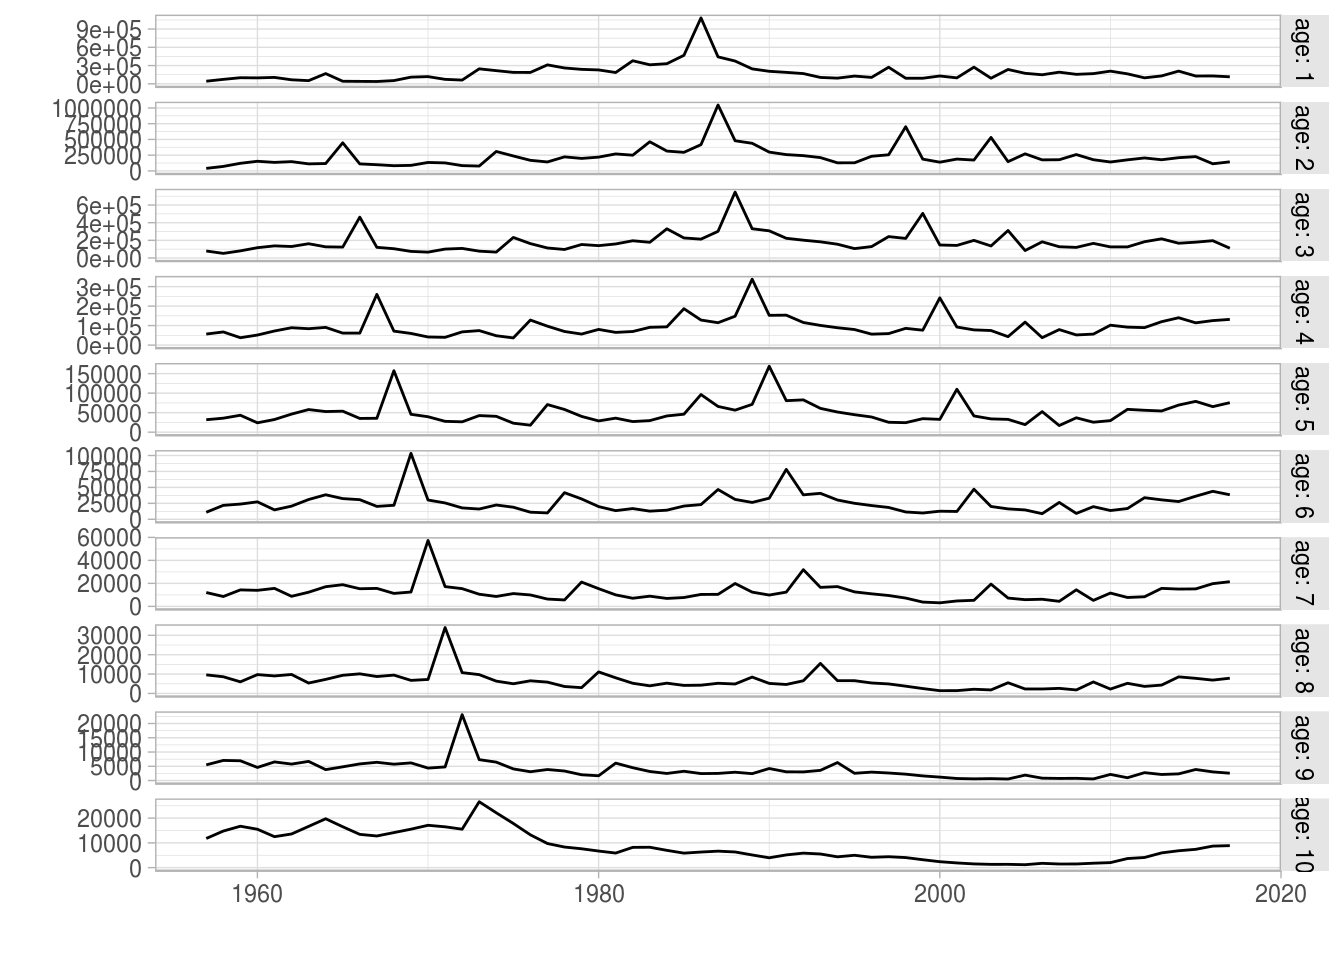
\includegraphics{docs/pdf/ggplotFL_plotting_FLR_objects_with_ggplot2_files/figure-latex/pflq-1} 

}

\caption{Standard ggplot2-based plot for an FLQuant object with multiple *year*s and *age*s.}\label{fig:pflq}
\end{figure}

For \texttt{FLQuant} objects with iterations, the \texttt{plot} method
will calculate, by default, the 50\% (median), 10\%, 25\%, 75\% and 90\%
quantiles, to be plotted as a solid line (50\%), a dotted line (10\%,
90\%) and a coloured ribbon (25\%-75\%).

\begin{Shaded}
\begin{Highlighting}[]
\KeywordTok{plot}\NormalTok{(}\KeywordTok{rlnorm}\NormalTok{(}\DecValTok{200}\NormalTok{, }\KeywordTok{fbar}\NormalTok{(ple4), }\FloatTok{0.15}\NormalTok{))}
\end{Highlighting}
\end{Shaded}

\begin{figure}

{\centering 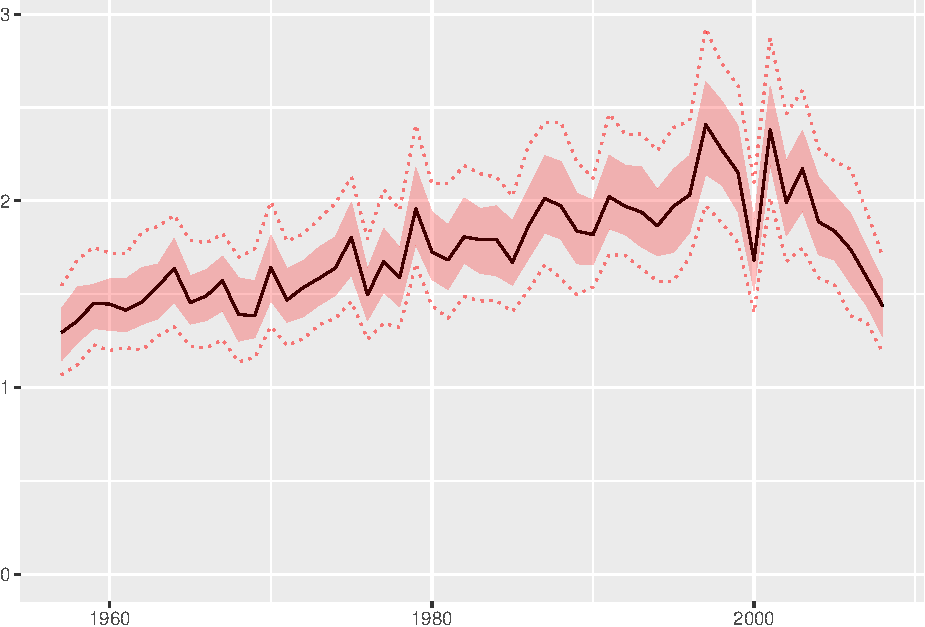
\includegraphics{docs/pdf/ggplotFL_plotting_FLR_objects_with_ggplot2_files/figure-latex/pflq2-1} 

}

\caption{Standard ggplot2-based plot for an FLQuant object with multiple iterations.}\label{fig:pflq2}
\end{figure}

Different quantiles can be specified using the \emph{probs} arguments,
and the alpha transparency of the ribbon will be proportional to the
probability value. A vector of odd length must be passed, and the
central point should be 0.50 so the central tendency line represents the
median. The most extreme quantiles will be plotted as dotted lines,
while all others will show up as ribbons.

\begin{Shaded}
\begin{Highlighting}[]
\KeywordTok{plot}\NormalTok{(}\KeywordTok{rlnorm}\NormalTok{(}\DecValTok{200}\NormalTok{, }\KeywordTok{fbar}\NormalTok{(ple4), }\FloatTok{0.15}\NormalTok{), }\DataTypeTok{probs=}\KeywordTok{c}\NormalTok{(}\FloatTok{0.05}\NormalTok{, }\FloatTok{0.10}\NormalTok{, }\FloatTok{0.25}\NormalTok{, }\FloatTok{0.50}\NormalTok{, }\FloatTok{0.75}\NormalTok{, }\FloatTok{0.90}\NormalTok{, }\FloatTok{0.95}\NormalTok{))}
\end{Highlighting}
\end{Shaded}

\begin{figure}

{\centering 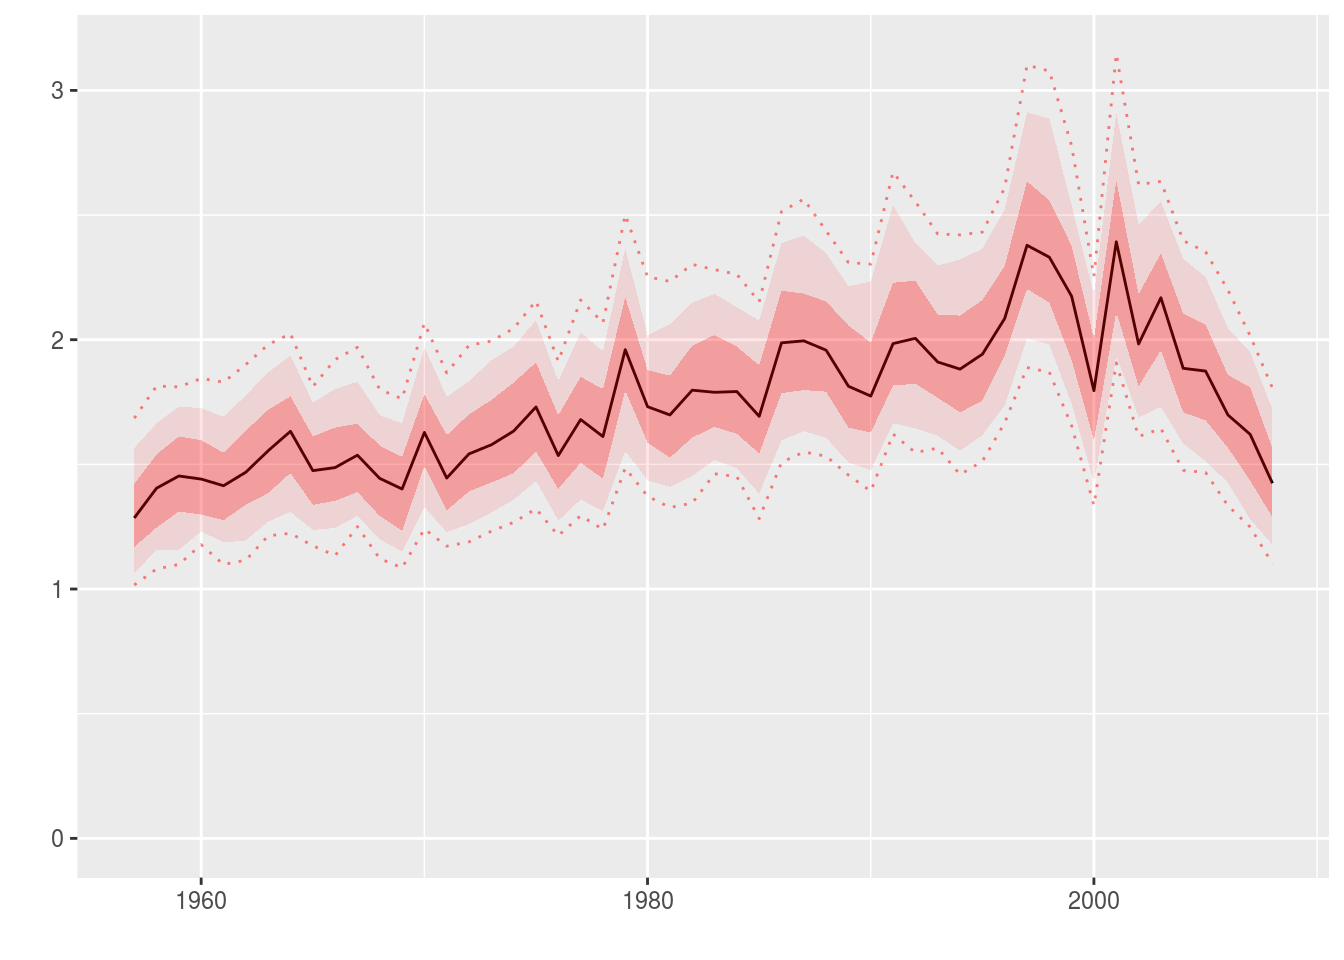
\includegraphics{docs/pdf/ggplotFL_plotting_FLR_objects_with_ggplot2_files/figure-latex/pflq3-1} 

}

\caption{Standard ggplot2-based plot for an FLQuant object with multiple iterations and user-specified quantiles.}\label{fig:pflq3}
\end{figure}

\subsection{\texorpdfstring{\texttt{FLQuants}}{FLQuants}}\label{flquants-1}

The \texttt{plot} method for \texttt{FLQuants} will now by default show
each object in a horizontal panel, with independent scales, by using
\texttt{facet\_grid}. Objects with iterations will have, as with
\texttt{plot} for \texttt{FLQuant}, their median, 10\%, 25\%, 75\% and
90\% quantiles shown as a black line and red ribbons with different
levels of transparency, respectively.

\begin{Shaded}
\begin{Highlighting}[]
\NormalTok{fqs <-}\StringTok{ }\KeywordTok{FLQuants}\NormalTok{(}\DataTypeTok{F =} \KeywordTok{rlnorm}\NormalTok{(}\DecValTok{200}\NormalTok{, }\KeywordTok{fbar}\NormalTok{(ple4), }\FloatTok{0.15}\NormalTok{), }\DataTypeTok{SSB =} \KeywordTok{ssb}\NormalTok{(ple4), }\DataTypeTok{Rec =} \KeywordTok{rec}\NormalTok{(ple4), }\DataTypeTok{Catch =} \KeywordTok{catch}\NormalTok{(ple4))}
\KeywordTok{plot}\NormalTok{(fqs)}
\end{Highlighting}
\end{Shaded}

\begin{figure}

{\centering 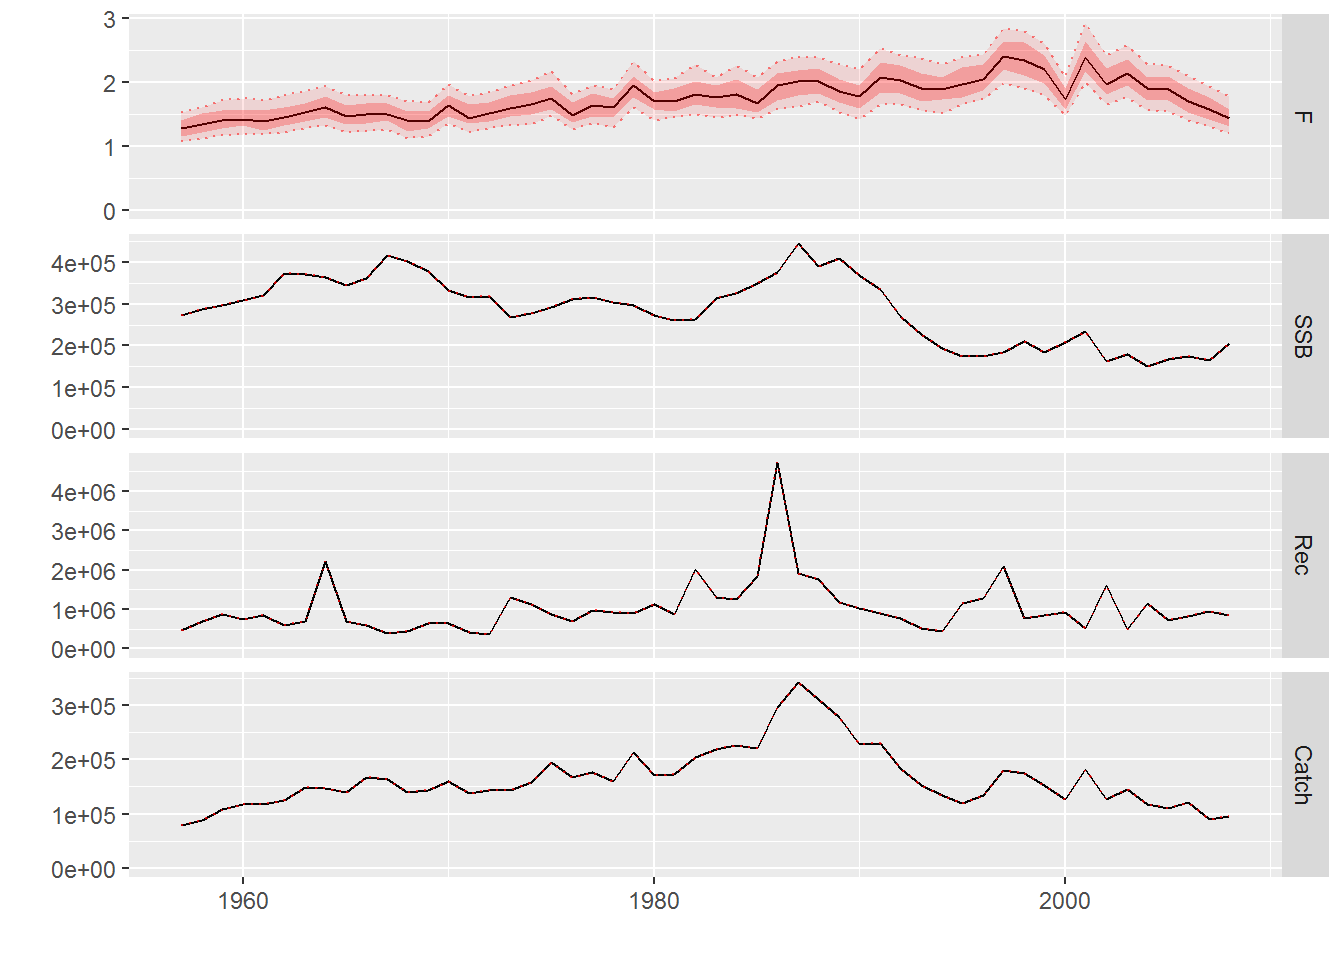
\includegraphics{docs/pdf/ggplotFL_plotting_FLR_objects_with_ggplot2_files/figure-latex/pflqs-1} 

}

\caption{Standard ggplot2-based plot for an FLQuants object with multiple iterations, and consisting of four elements.}\label{fig:pflqs}
\end{figure}

Plots of multiple \texttt{FLQuant} objects use by default
\texttt{facet\_grid} with multiple plots stacked on top of each other.
To have the plots on a grid, you can add a call to \texttt{facet\_wrap}
to change it. For example, here we have a 2x2 grid

\begin{Shaded}
\begin{Highlighting}[]
\NormalTok{fqs <-}\StringTok{ }\KeywordTok{FLQuants}\NormalTok{(}\DataTypeTok{F =} \KeywordTok{rlnorm}\NormalTok{(}\DecValTok{200}\NormalTok{, }\KeywordTok{fbar}\NormalTok{(ple4), }\FloatTok{0.15}\NormalTok{), }\DataTypeTok{SSB =} \KeywordTok{ssb}\NormalTok{(ple4), }\DataTypeTok{Rec =} \KeywordTok{rec}\NormalTok{(ple4), }\DataTypeTok{Catch =} \KeywordTok{catch}\NormalTok{(ple4))}
\KeywordTok{plot}\NormalTok{(fqs) +}\StringTok{ }\KeywordTok{facet_wrap}\NormalTok{(~qname, }\DataTypeTok{scales=}\StringTok{"free"}\NormalTok{)}
\end{Highlighting}
\end{Shaded}

\begin{figure}

{\centering 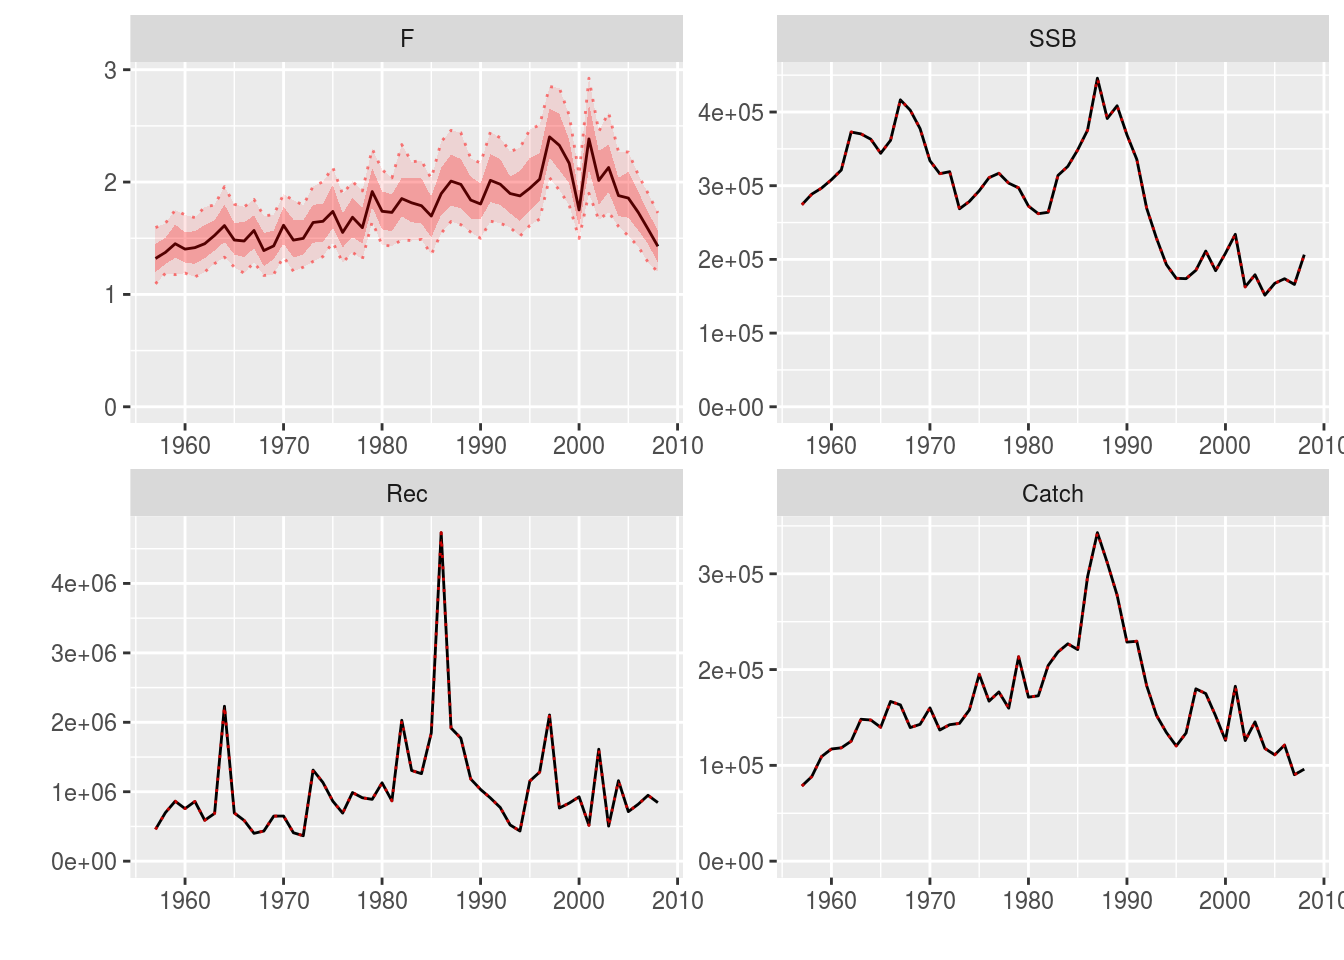
\includegraphics{docs/pdf/ggplotFL_plotting_FLR_objects_with_ggplot2_files/figure-latex/pflqsg-1} 

}

\caption{Wrap-based ggplot2-based plot for an FLQuants object with multiple iterations, and consisting of four elements.}\label{fig:pflqsg}
\end{figure}

\subsection{\texorpdfstring{\texttt{FLStock}}{FLStock}}\label{flstock-1}

The \texttt{ggplotFL} version of the standard plot for the
\texttt{FLStock} class contains the time series of recruitment (obtained
by calling \texttt{rec()}), SSB (\texttt{ssb()}), catch
(\texttt{catch()}), and fishing mortality or harvest for selected
ages(\texttt{fbar()}). The four panels are now arranged in a 4-row
matrix to better display the trends in the time series.

\begin{Shaded}
\begin{Highlighting}[]
\KeywordTok{plot}\NormalTok{(ple4)}
\end{Highlighting}
\end{Shaded}

\begin{figure}

{\centering 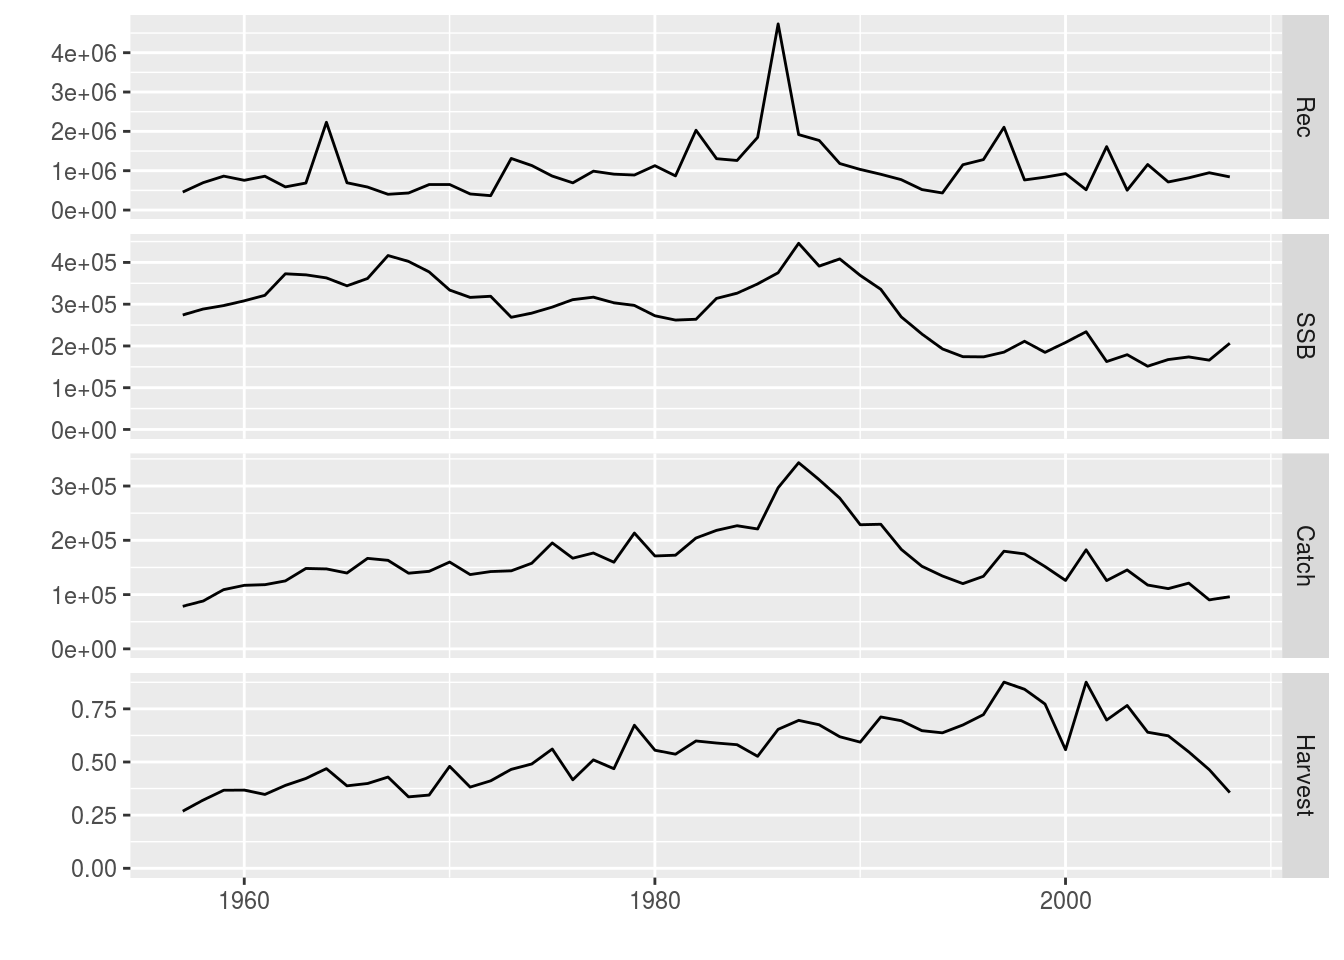
\includegraphics{docs/pdf/ggplotFL_plotting_FLR_objects_with_ggplot2_files/figure-latex/pfls-1} 

}

\caption{A ggplot2 version of the standard plot() for FLStock, as applied to `ple4`}\label{fig:pfls}
\end{figure}

\subsection{\texorpdfstring{\texttt{FLStocks}}{FLStocks}}\label{flstocks}

Similarly, the standard \texttt{plot()} method for the \texttt{FLStocks}
class now relies on \texttt{ggplot}. For example, we can create an
example \texttt{FLStocks} object by splitting the female and male units
of \texttt{ple4sex} and adding them as separate elements in the list. A
call to \texttt{plot()} would give us the corresponding plot. Remember
the object returned by \texttt{ggplot} can always be assigned to a
variable in the workspace and modified as required (see examples below).

\begin{Shaded}
\begin{Highlighting}[]
\KeywordTok{plot}\NormalTok{(}\KeywordTok{FLStocks}\NormalTok{(}\DataTypeTok{Male=}\NormalTok{ple4sex[,,}\StringTok{'male'}\NormalTok{], }\DataTypeTok{Female=}\NormalTok{ple4sex[,,}\StringTok{'female'}\NormalTok{])) +}\StringTok{ }\KeywordTok{theme}\NormalTok{(}\DataTypeTok{legend.position=}\StringTok{"top"}\NormalTok{)}
\end{Highlighting}
\end{Shaded}

\begin{figure}

{\centering 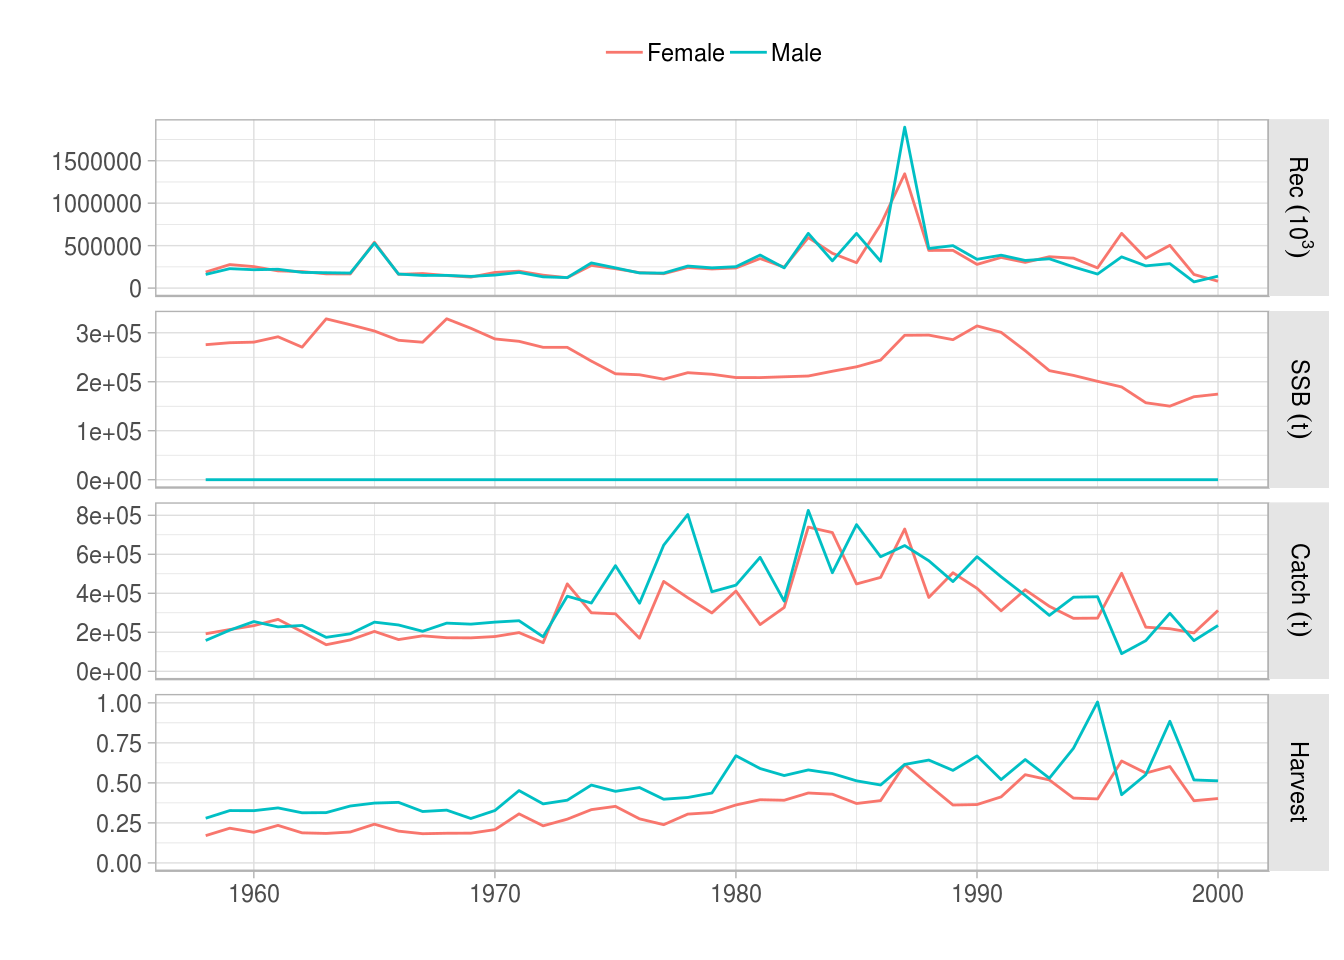
\includegraphics{docs/pdf/ggplotFL_plotting_FLR_objects_with_ggplot2_files/figure-latex/pflss-1} 

}

\caption{ggplot2 version of the standard plot() for FLStocks, as applied to the sex-separated FLStock object `ple4sex`}\label{fig:pflss}
\end{figure}

\subsection{\texorpdfstring{\texttt{FLSR}}{FLSR}}\label{flsr}

The \texttt{ggplotFL} version of the class plot for \texttt{FLSR}
contains the same six panels as before:

\begin{enumerate}
\def\labelenumi{(\arabic{enumi})}
\tightlist
\item
  stock-recruit data, fitted model and lowess smoother,
\item
  residuals by year,
\item
  lag 1-correlated residuals,
\item
  residuals by SSB,
\item
  residuals qqplot, and
\item
  residuals by fitted values.
\end{enumerate}

Blue lines are lowess smoothers, to better visualize trends in the data
shown.

\begin{Shaded}
\begin{Highlighting}[]
\KeywordTok{plot}\NormalTok{(nsher)}
\end{Highlighting}
\end{Shaded}

\begin{figure}

{\centering 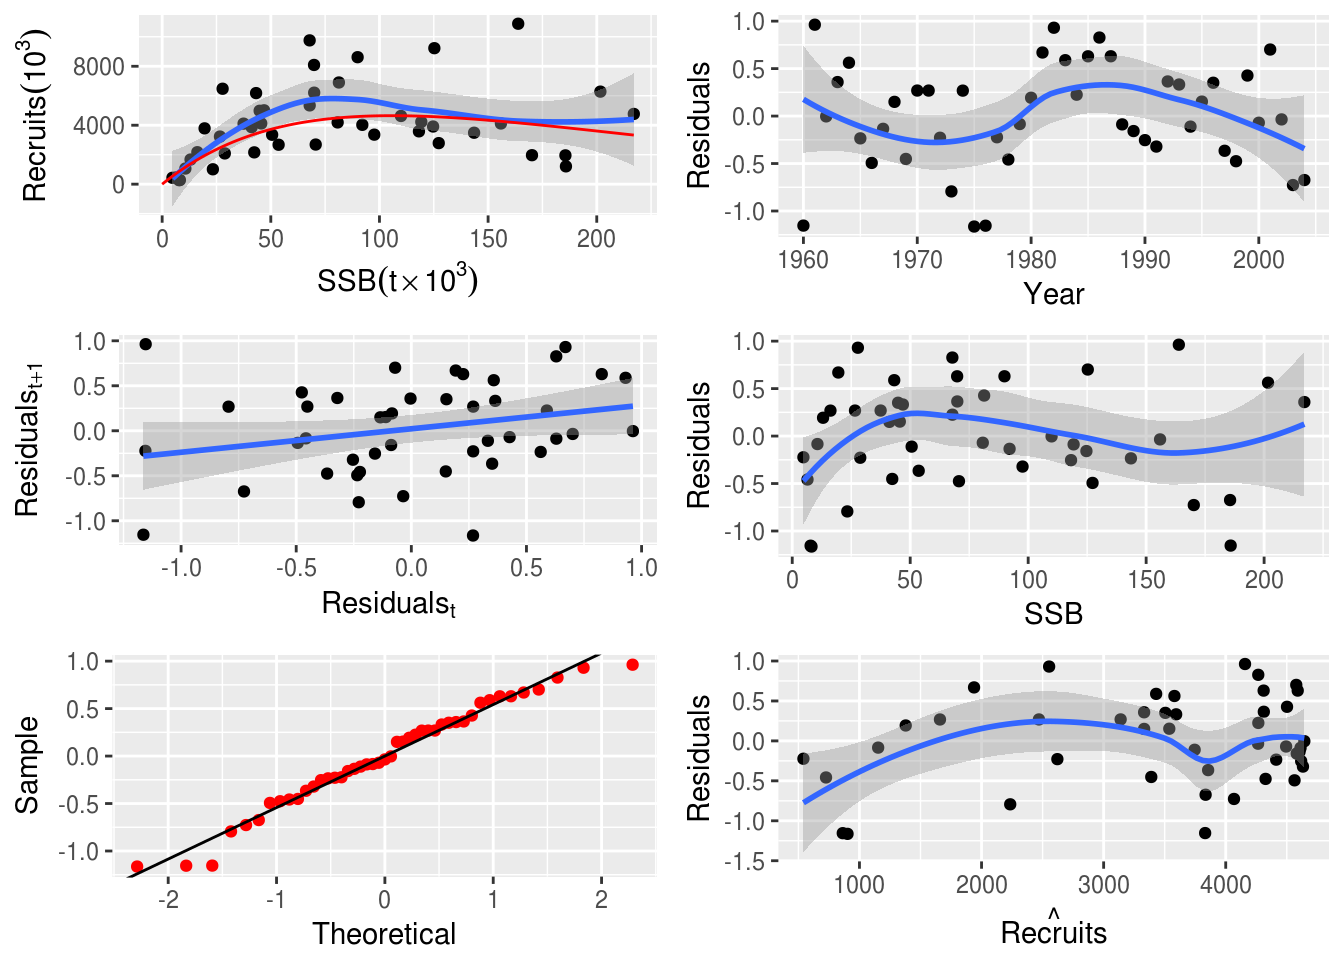
\includegraphics{docs/pdf/ggplotFL_plotting_FLR_objects_with_ggplot2_files/figure-latex/pflsr-1} 

}

\caption{Standard ggplot2-based plot for an object of class FLSR.}\label{fig:pflsr}
\end{figure}

\subsection{\texorpdfstring{\texttt{FLSRs}}{FLSRs}}\label{flsrs}

A class plot also exists for \texttt{FLSRs} objects, lists with
\texttt{FLSR} elements. The comparison shown involves only the model fit
across the different model functions or formulations, but not the
residuals diagnostics available for \texttt{FLSR}. The default legend
contains the formula of each of the fitted models and the parameter
values (or the median if multiple iterations exist).

\begin{Shaded}
\begin{Highlighting}[]
\NormalTok{srs <-}\StringTok{ }\KeywordTok{FLSRs}\NormalTok{(}\KeywordTok{sapply}\NormalTok{(}\KeywordTok{c}\NormalTok{(}\StringTok{'ricker'}\NormalTok{, }\StringTok{'bevholt'}\NormalTok{), function(x) \{}
         \NormalTok{y <-}\StringTok{ }\NormalTok{nsher}
         \KeywordTok{model}\NormalTok{(y) <-}\StringTok{ }\NormalTok{x}
         \KeywordTok{return}\NormalTok{(}\KeywordTok{fmle}\NormalTok{(y))\}))}
\end{Highlighting}
\end{Shaded}

\begin{Shaded}
\begin{Highlighting}[]
\KeywordTok{plot}\NormalTok{(srs)}
\end{Highlighting}
\end{Shaded}

\begin{figure}

{\centering 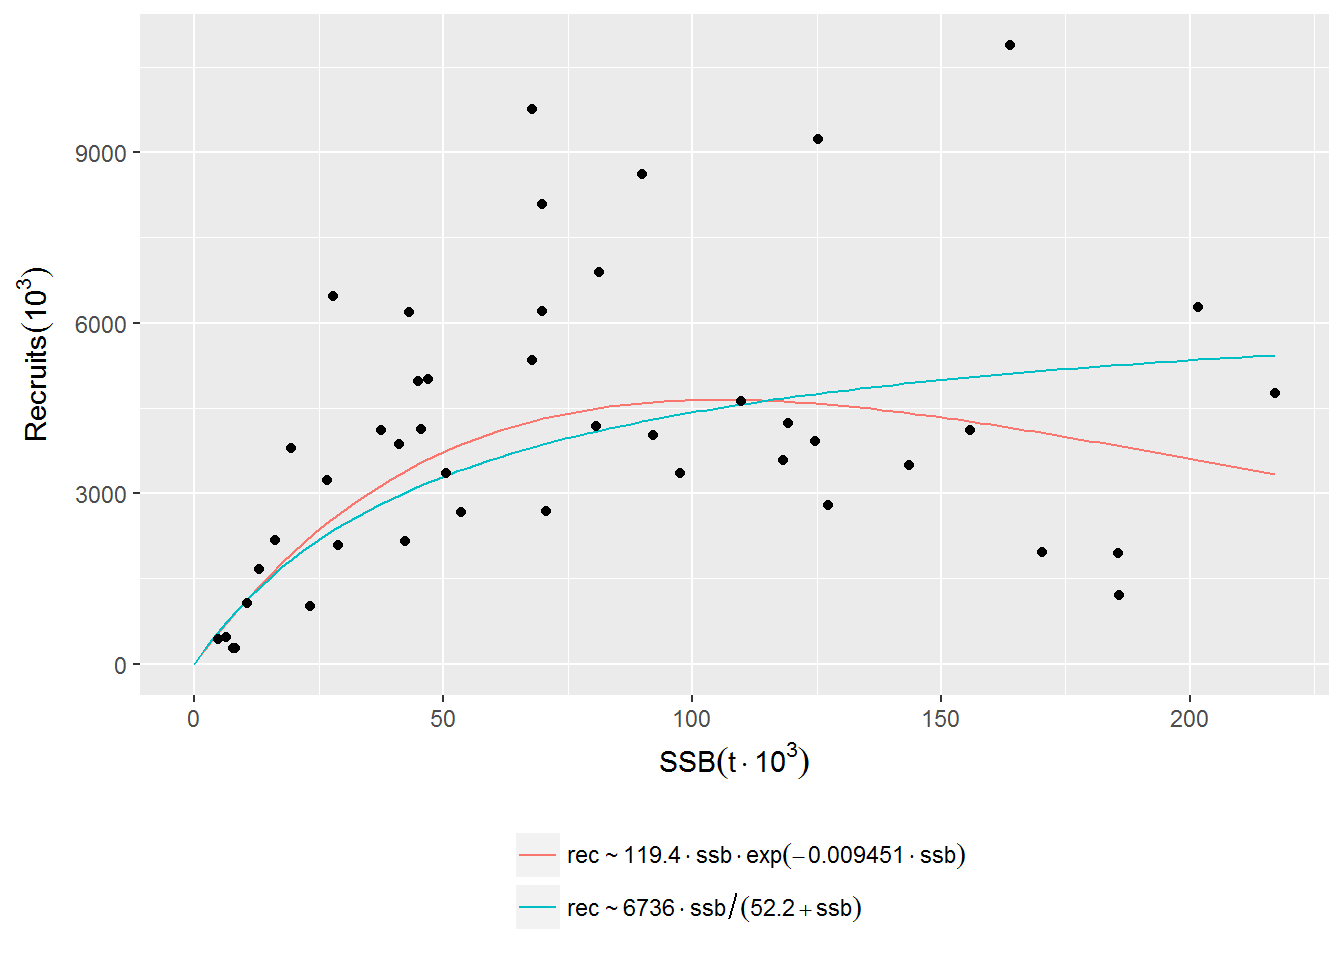
\includegraphics{docs/pdf/ggplotFL_plotting_FLR_objects_with_ggplot2_files/figure-latex/pflsrs-1} 

}

\caption{Standard ggplot2-based plot for an FLSRs object, using default legend labels.}\label{fig:pflsrs}
\end{figure}

An alternative labeller function exists (\emph{modlabel}) that returns
the name of the SR model function and the parameter values, by using the
\emph{legend\_label} argument.

\begin{Shaded}
\begin{Highlighting}[]
\KeywordTok{plot}\NormalTok{(srs, }\DataTypeTok{legend_label=}\NormalTok{modlabel) }
\end{Highlighting}
\end{Shaded}

\begin{figure}

{\centering 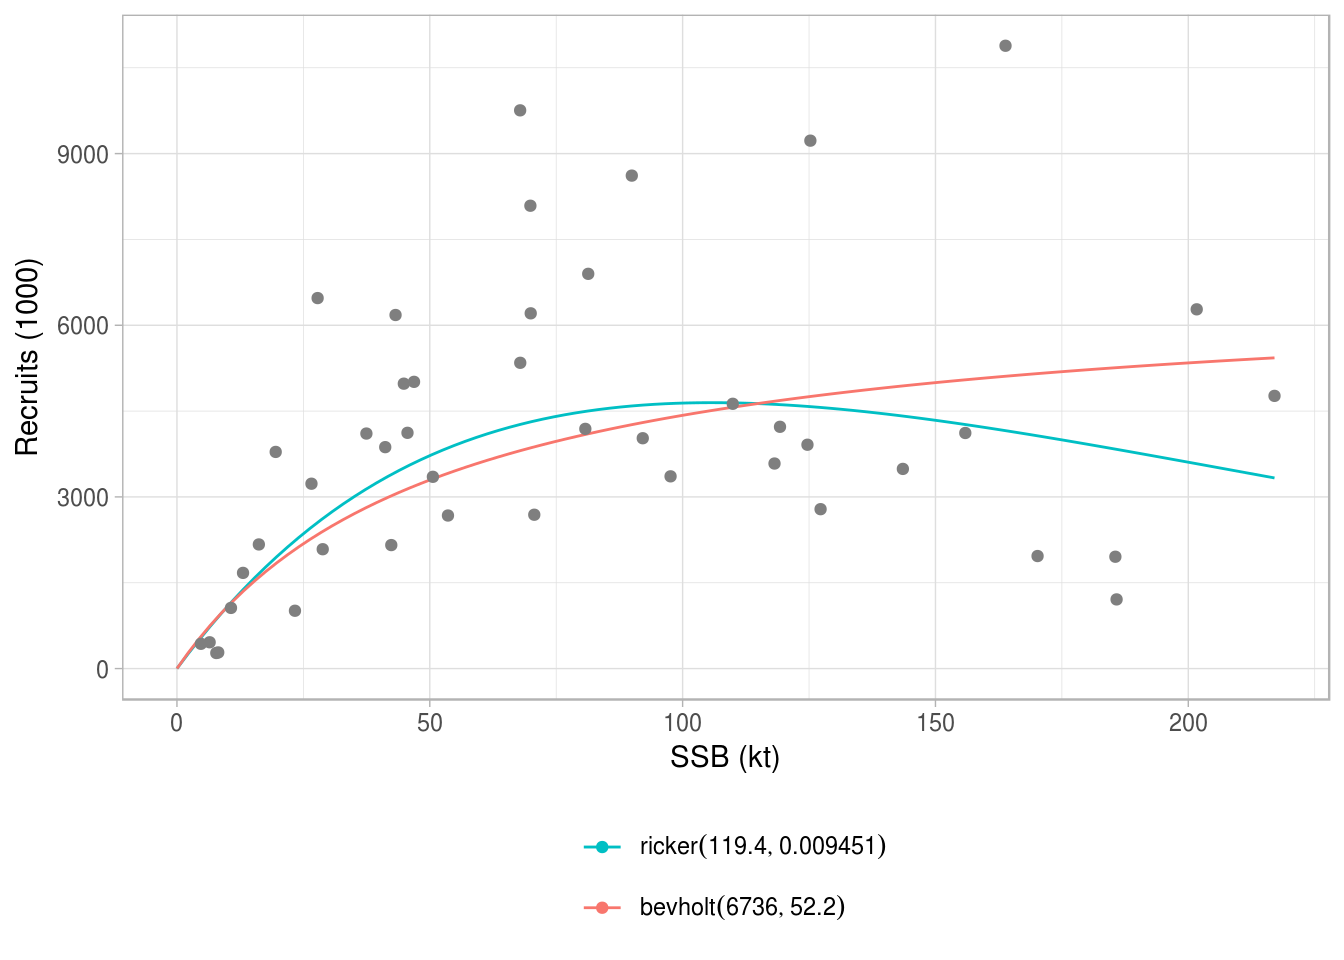
\includegraphics{docs/pdf/ggplotFL_plotting_FLR_objects_with_ggplot2_files/figure-latex/pflsrs2-1} 

}

\caption{Standard ggplot2-based plot for an FLSRs object, using model names as legend labels.}\label{fig:pflsrs2}
\end{figure}

As is common in \texttt{ggplot2}, labels can be specified directly,
overwriting those included in the method. You should ignore the warning
about scale for \emph{color} being replaced.

\begin{Shaded}
\begin{Highlighting}[]
\KeywordTok{plot}\NormalTok{(srs) +}\StringTok{ }\KeywordTok{scale_color_discrete}\NormalTok{(}\DataTypeTok{name=}\StringTok{"SR models"}\NormalTok{, }\DataTypeTok{breaks=}\KeywordTok{c}\NormalTok{(}\StringTok{'ricker'}\NormalTok{, }\StringTok{'bevholt'}\NormalTok{),}
\DataTypeTok{labels=}\KeywordTok{c}\NormalTok{(}\StringTok{"Ricker"}\NormalTok{, }\StringTok{"Beverton & Holt"}\NormalTok{))}
\end{Highlighting}
\end{Shaded}

\begin{figure}

{\centering 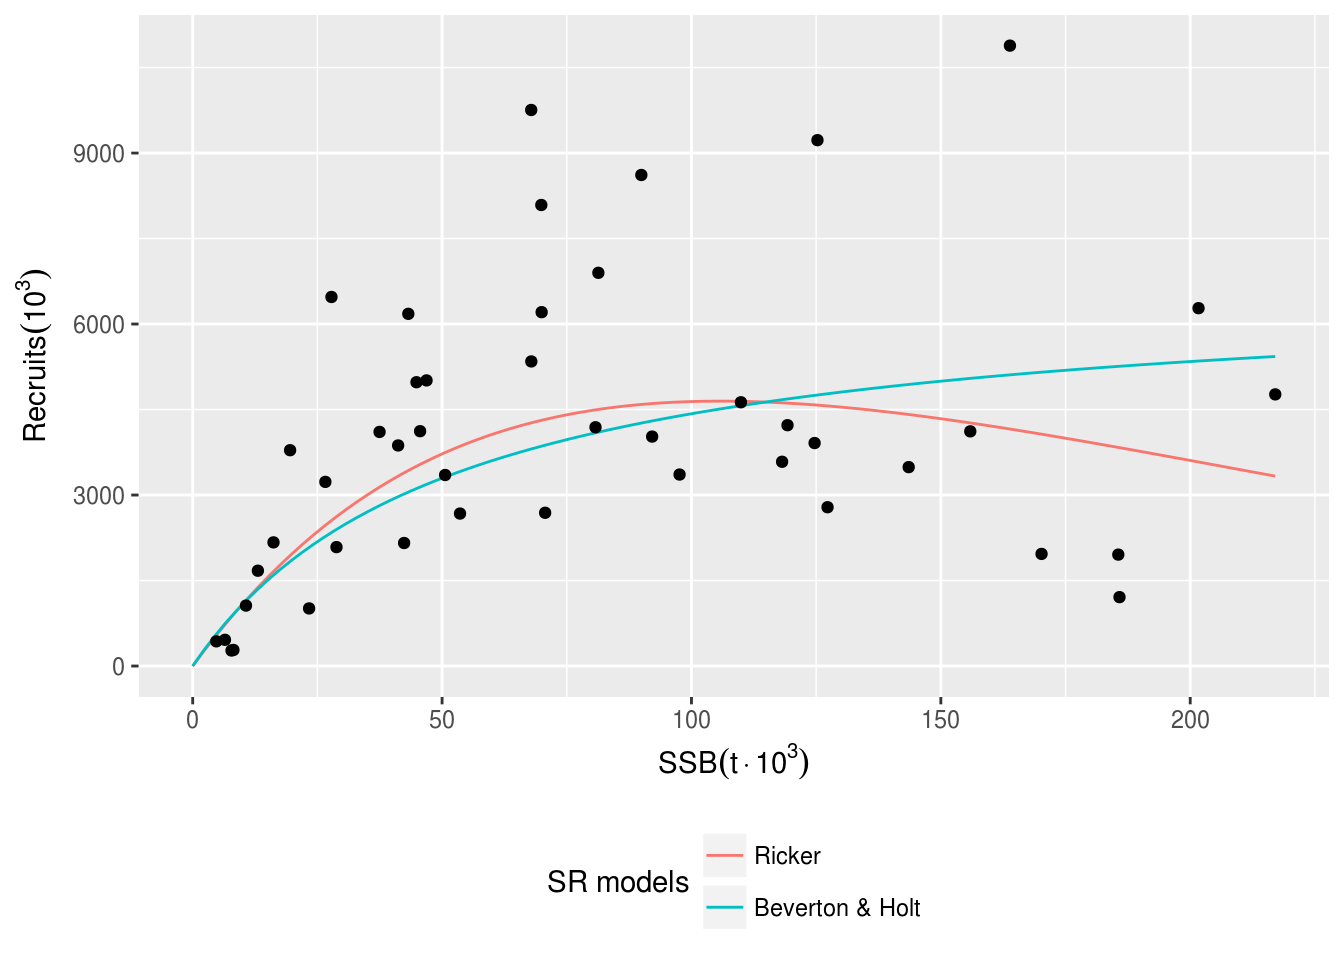
\includegraphics{docs/pdf/ggplotFL_plotting_FLR_objects_with_ggplot2_files/figure-latex/pflsrs3-1} 

}

\caption{Standard ggplot2-based plot for an FLSRs object, using model names as legend labels.}\label{fig:pflsrs3}
\end{figure}

\section{\texorpdfstring{Using \texttt{ggplot2} directly by converting
to
\texttt{data.frame}}{Using ggplot2 directly by converting to data.frame}}\label{using-ggplot2-directly-by-converting-to-data.frame}

The methods shown above depend on conversion of \emph{FLR} objects into
\texttt{data.frame}, which can then be passed to \texttt{ggplot()}.
Calling \texttt{ggplot} on an \emph{FLR} object takes care of this
conversion behind the scenes, but to obtain full control and develop
certains plots, it is best to explicitely convert the \emph{FLR} objects
into a \texttt{data.frame}. Different conventions are used in the naming
of the dataframe columns created from various \emph{FLR} classes, which
need to be used when the plot is specified. For further information,
please see the help pages for each \texttt{data.frame()} method
\footnote{For example
  \texttt{method?as.data.frame(\textquotesingle{}FLQuants\textquotesingle{})}}.

\section{Some examples}\label{some-examples}

\subsection{Example: plot quantiles of a
simulation}\label{example-plot-quantiles-of-a-simulation}

To have full control over a plot of the median (or mean) and the
confidence or probability intervals of a simulated or randomized time
series, i.e.~an \texttt{FLQuant} object with iters, we need to arrange
the different values computed from the object in separate columns of a
\texttt{data.frame}.

If we start with some random \texttt{FLQuant} object, such as

\begin{Shaded}
\begin{Highlighting}[]
\NormalTok{fla <-}\StringTok{ }\KeywordTok{rlnorm}\NormalTok{(}\DecValTok{100}\NormalTok{, }\KeywordTok{FLQuant}\NormalTok{(}\KeywordTok{exp}\NormalTok{(}\KeywordTok{cumsum}\NormalTok{(}\KeywordTok{rnorm}\NormalTok{(}\DecValTok{25}\NormalTok{, }\DecValTok{0}\NormalTok{, }\FloatTok{0.1}\NormalTok{)))), }\FloatTok{0.1}\NormalTok{) }
\KeywordTok{ggplot}\NormalTok{(fla, }\KeywordTok{aes}\NormalTok{(}\KeywordTok{factor}\NormalTok{(year), data)) +}\StringTok{ }\KeywordTok{geom_boxplot}\NormalTok{() +}\StringTok{ }\KeywordTok{xlab}\NormalTok{(}\StringTok{""}\NormalTok{)}
\end{Highlighting}
\end{Shaded}

\begin{figure}

{\centering 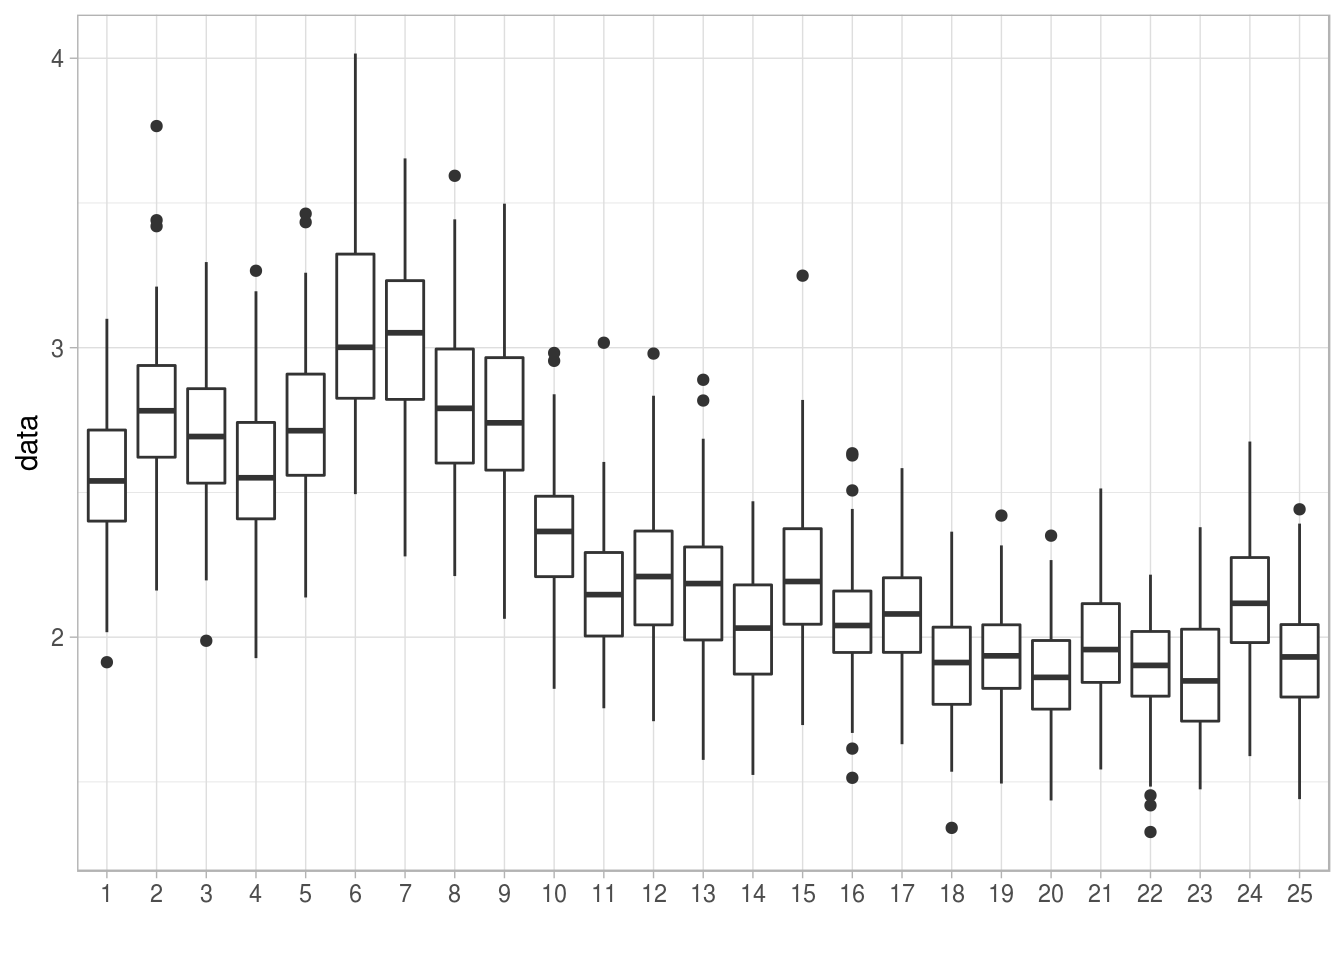
\includegraphics{docs/pdf/ggplotFL_plotting_FLR_objects_with_ggplot2_files/figure-latex/exsim1-1} 

}

\caption{Distribution of values of a simulated time series plotted using geom_boxplot()}\label{fig:exsim1}
\end{figure}

We can first compute the necessary statistics on the object itself, as
these operations are very efficient on an array. \texttt{quantile()} on
an \texttt{FLQuant} will return the specified quantiles along the iter
dimension. Let's extract the 10th, 25th, 50th, 75th and 90th quantiles.

\begin{Shaded}
\begin{Highlighting}[]
\NormalTok{flq <-}\StringTok{ }\KeywordTok{quantile}\NormalTok{(fla, }\KeywordTok{c}\NormalTok{(}\FloatTok{0.10}\NormalTok{, }\FloatTok{0.25}\NormalTok{, }\FloatTok{0.50}\NormalTok{, }\FloatTok{0.75}\NormalTok{, }\FloatTok{0.90}\NormalTok{))}
\end{Highlighting}
\end{Shaded}

The object can now be coerced to a \texttt{data.frame} and inspected to
see how the 100 iters have now been turned into the five requested
quantiles in the iter column

\begin{Shaded}
\begin{Highlighting}[]
\NormalTok{fdf <-}\StringTok{ }\KeywordTok{as.data.frame}\NormalTok{(flq, }\DataTypeTok{drop=}\OtherTok{TRUE}\NormalTok{)}
\KeywordTok{head}\NormalTok{(fdf, }\DecValTok{3}\NormalTok{)}
\end{Highlighting}
\end{Shaded}

\begin{longtable}[c]{@{}rlr@{}}
\toprule
year & iter & data\tabularnewline
\midrule
\endhead
1 & 10\% & 2.238\tabularnewline
2 & 10\% & 2.432\tabularnewline
3 & 10\% & 2.379\tabularnewline
\bottomrule
\end{longtable}

The long-format \texttt{data.frame} can be reshaped into a wide-format
one so that we can instruct \texttt{ggplot} to use the quantiles, now in
separate columns, to provide limits for the shaded areas in
\emph{geom\_ribbon}. To do this we can use \texttt{reshape}, as follows

\begin{Shaded}
\begin{Highlighting}[]
\NormalTok{fdw <-}\StringTok{ }\KeywordTok{reshape}\NormalTok{(fdf, }\DataTypeTok{timevar =} \StringTok{"iter"}\NormalTok{, }\DataTypeTok{idvar =} \KeywordTok{c}\NormalTok{(}\StringTok{"year"}\NormalTok{), }\DataTypeTok{direction =} \StringTok{"wide"}\NormalTok{)}
\end{Highlighting}
\end{Shaded}

This creates a wide \texttt{data.frame} in which the iter column is
spread into five columns named as the levels of its conversion into
factor

\begin{Shaded}
\begin{Highlighting}[]
\KeywordTok{levels}\NormalTok{(fdf[,}\StringTok{'iter'}\NormalTok{])}
\end{Highlighting}
\end{Shaded}

\begin{verbatim}
[1] "10%" "25%" "50%" "75%" "90%"
\end{verbatim}

We can now use those five quantile columns when plotting shaded areas
using \emph{geom\_ribbon}. Please note that the column names returned by
\texttt{quantile()} need to be quoted using backticks.

\begin{Shaded}
\begin{Highlighting}[]
\NormalTok{p <-}\StringTok{ }\KeywordTok{ggplot}\NormalTok{(}\DataTypeTok{data=}\NormalTok{fdw, }\KeywordTok{aes}\NormalTok{(}\DataTypeTok{x=}\NormalTok{year, }\DataTypeTok{y=}\StringTok{`}\DataTypeTok{data.50%}\StringTok{`}\NormalTok{)) +}
\KeywordTok{geom_ribbon}\NormalTok{(}\KeywordTok{aes}\NormalTok{(}\DataTypeTok{x=}\NormalTok{year, }\DataTypeTok{ymin =} \StringTok{`}\DataTypeTok{data.10%}\StringTok{`}\NormalTok{, }\DataTypeTok{ymax =} \StringTok{`}\DataTypeTok{data.90%}\StringTok{`}\NormalTok{), }\DataTypeTok{fill=}\StringTok{"red"}\NormalTok{, }\DataTypeTok{alpha =} \NormalTok{.}\DecValTok{15}\NormalTok{) +}
\KeywordTok{geom_ribbon}\NormalTok{(}\KeywordTok{aes}\NormalTok{(}\DataTypeTok{x=}\NormalTok{year, }\DataTypeTok{ymin =} \StringTok{`}\DataTypeTok{data.25%}\StringTok{`}\NormalTok{, }\DataTypeTok{ymax =} \StringTok{`}\DataTypeTok{data.75%}\StringTok{`}\NormalTok{), }\DataTypeTok{fill=}\StringTok{"red"}\NormalTok{, }\DataTypeTok{alpha =} \NormalTok{.}\DecValTok{25}\NormalTok{) +}
\KeywordTok{geom_line}\NormalTok{() +}\StringTok{ }\KeywordTok{ylab}\NormalTok{(}\StringTok{"data"}\NormalTok{)}
\KeywordTok{print}\NormalTok{(p)}
\end{Highlighting}
\end{Shaded}

\textbackslash{}begin\{figure\}

\{\centering 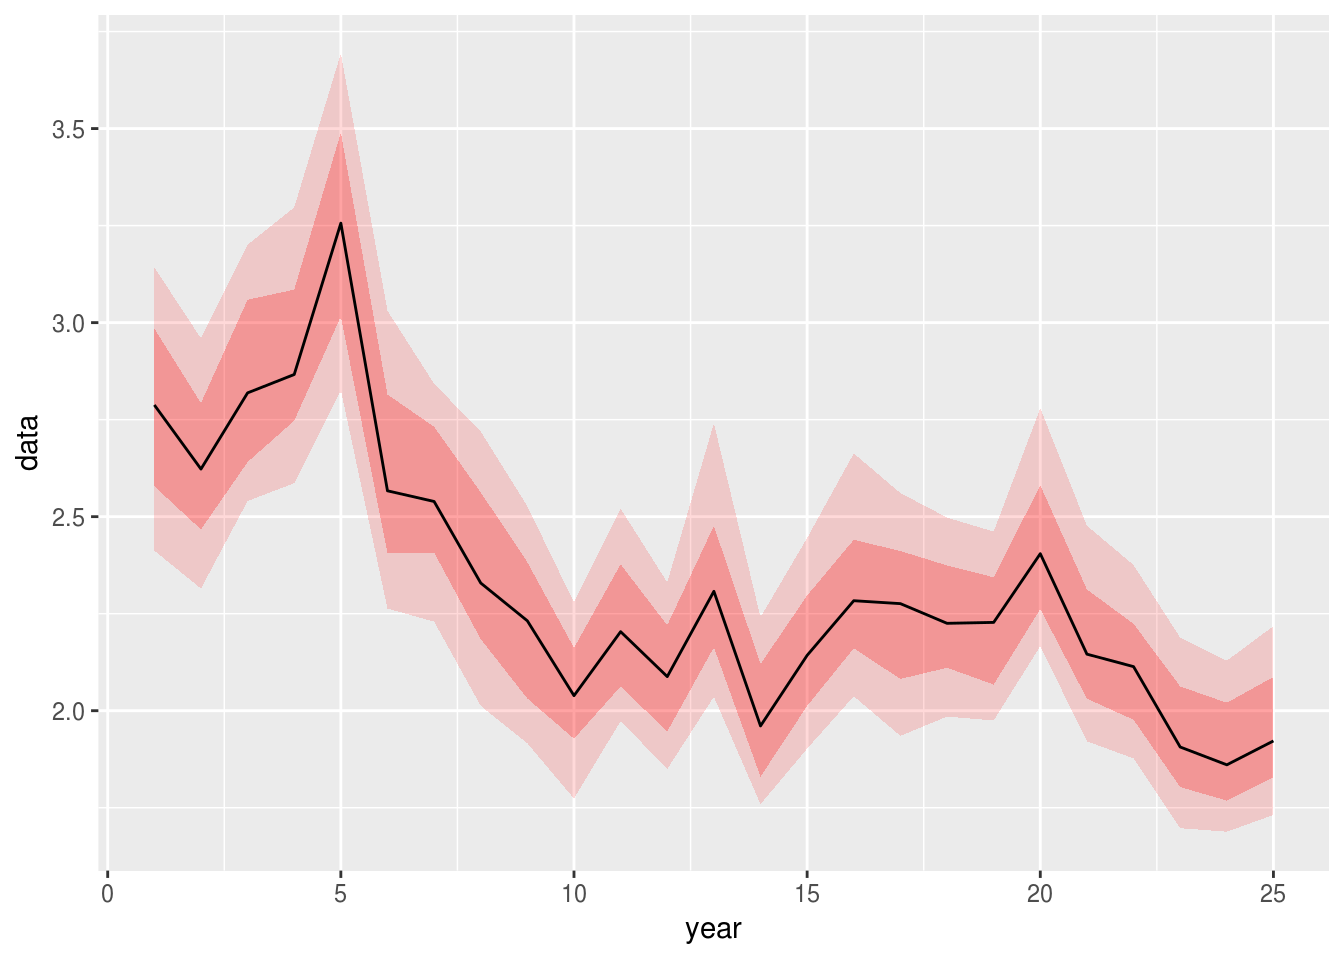
\includegraphics{docs/pdf/ggplotFL_plotting_FLR_objects_with_ggplot2_files/figure-latex/exsim6-1}

\}

\textbackslash{}caption\{Time series with 75\% and 90\% credibility
intervals plotted using geom\_ribbon.\}\label{fig:exsim6}
\textbackslash{}end\{figure\}

Assigning the result of the call to \texttt{ggplot()} to a variable, as
done above, will allow us to reuse the plot later on by modifying or
adding components.

\subsection{Example: Simulation trajectories
plot}\label{example-simulation-trajectories-plot}

If the result of a stochastic simulation is summarised by showing
credibility intervals, it is very informative to plot as well some of
the individual iterations (in this case we want iteration 1, 4 and 23)
as a way of showing the fact that individual trajectories are generally
not as smooth as, for example, the median shown in the figure above.

\begin{Shaded}
\begin{Highlighting}[]
\NormalTok{fds  <-}\StringTok{ }\KeywordTok{as.data.frame}\NormalTok{(}\KeywordTok{iter}\NormalTok{(fla, }\KeywordTok{c}\NormalTok{(}\DecValTok{1}\NormalTok{, }\DecValTok{4}\NormalTok{, }\DecValTok{23}\NormalTok{)))}
\NormalTok{p +}\StringTok{ }\KeywordTok{geom_line}\NormalTok{(}\DataTypeTok{data=}\NormalTok{fds, }\KeywordTok{aes}\NormalTok{(year, data, }\DataTypeTok{colour=}\NormalTok{iter), }\DataTypeTok{size=}\FloatTok{0.5}\NormalTok{) +}\StringTok{ }
\StringTok{  }\KeywordTok{theme}\NormalTok{(}\DataTypeTok{legend.position =} \StringTok{"none"}\NormalTok{)}
\end{Highlighting}
\end{Shaded}

\begin{figure}

{\centering 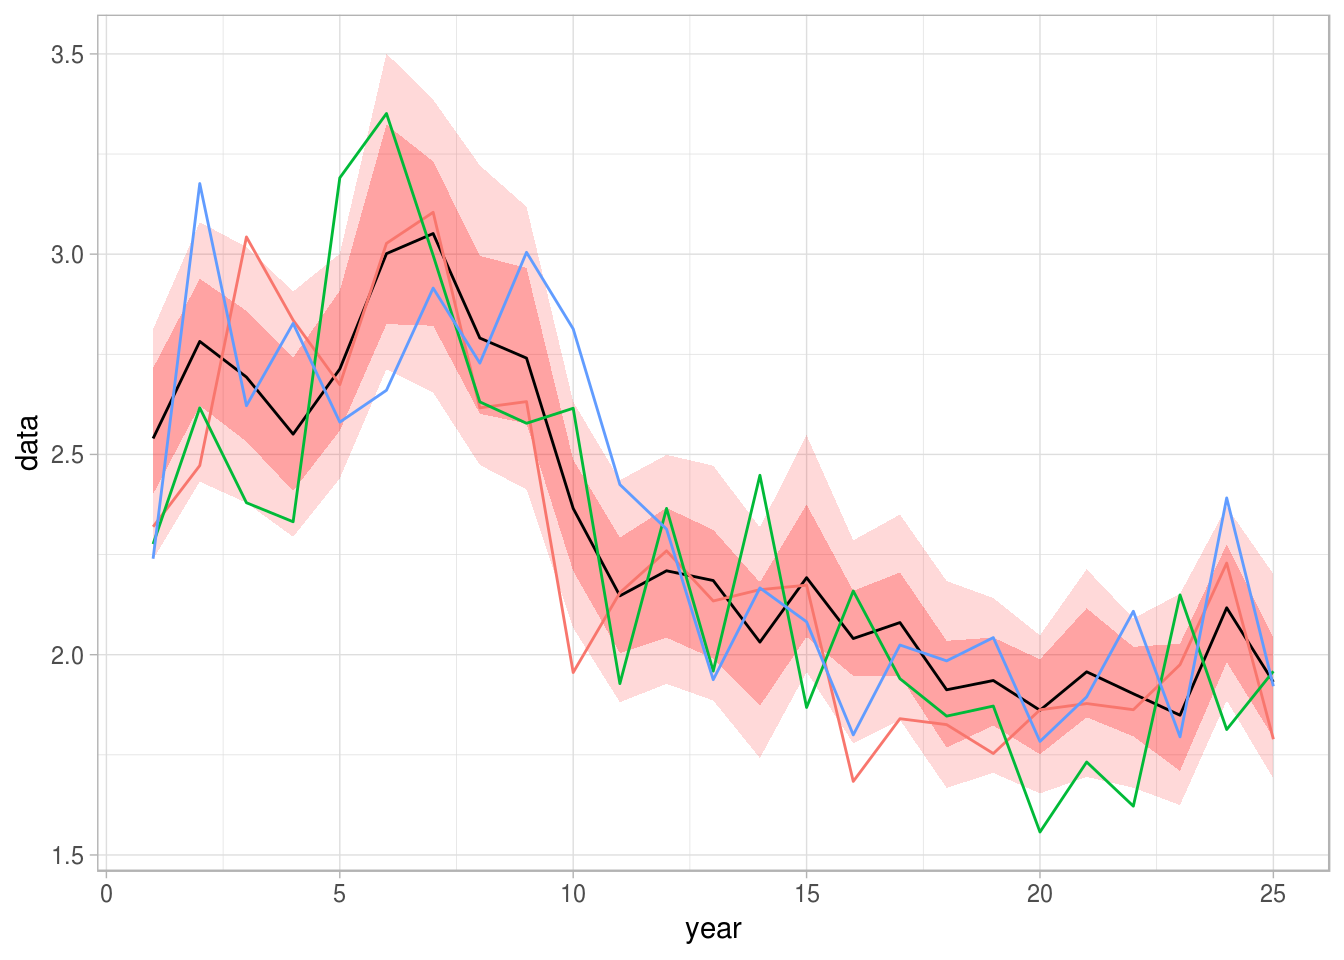
\includegraphics{docs/pdf/ggplotFL_plotting_FLR_objects_with_ggplot2_files/figure-latex/exspa-1} 

}

\caption{Spaghetti plot of a stochastic simulation, by calling geom_line on top of the stored ribbon plot.}\label{fig:exspa}
\end{figure}

This is easy to do in \texttt{ggplot2} by adding an extra element on top
of the previous plot, stored in the \texttt{p} object from the code
above.

\subsection{\texorpdfstring{Example: Using
\texttt{FLQuants}}{Example: Using FLQuants}}\label{example-using-flquants}

Coercion using \texttt{as.data.frame}, combined with the use of
\texttt{reshape}, or \texttt{dcast} and \texttt{melt} (from the
\texttt{reshape2} package\footnote{\url{http://cran.r-project.org/package=reshape2}}),
provides the \emph{FLR} user with the tools required to create a large
range of \texttt{ggplot}s from any \emph{FLR} object.

\textbf{TODO}: ADD text \& example

\subsection{Example: Bubble plots}\label{example-bubble-plots}

Bubble plots allow us to represent a third continuous dimension in a
scatter plot by sizing points according the value of a variable. For
example, catch in numbers by age and year can be visualised using

\begin{Shaded}
\begin{Highlighting}[]
\KeywordTok{ggplot}\NormalTok{(}\KeywordTok{catch.n}\NormalTok{(ple4), }\KeywordTok{aes}\NormalTok{(year, }\KeywordTok{as.factor}\NormalTok{(age), }\DataTypeTok{size=}\NormalTok{data)) +}\StringTok{ }\KeywordTok{geom_point}\NormalTok{(}\DataTypeTok{shape=}\DecValTok{21}\NormalTok{) +}\StringTok{ }
\StringTok{  }\KeywordTok{scale_size}\NormalTok{(}\DataTypeTok{range =} \KeywordTok{c}\NormalTok{(}\DecValTok{1}\NormalTok{, }\DecValTok{20}\NormalTok{)) +}\StringTok{ }\KeywordTok{ylab}\NormalTok{(}\StringTok{"age"}\NormalTok{) +}\StringTok{ }\KeywordTok{theme}\NormalTok{(}\DataTypeTok{legend.position =} \StringTok{"none"}\NormalTok{)}
\end{Highlighting}
\end{Shaded}

\begin{figure}

{\centering 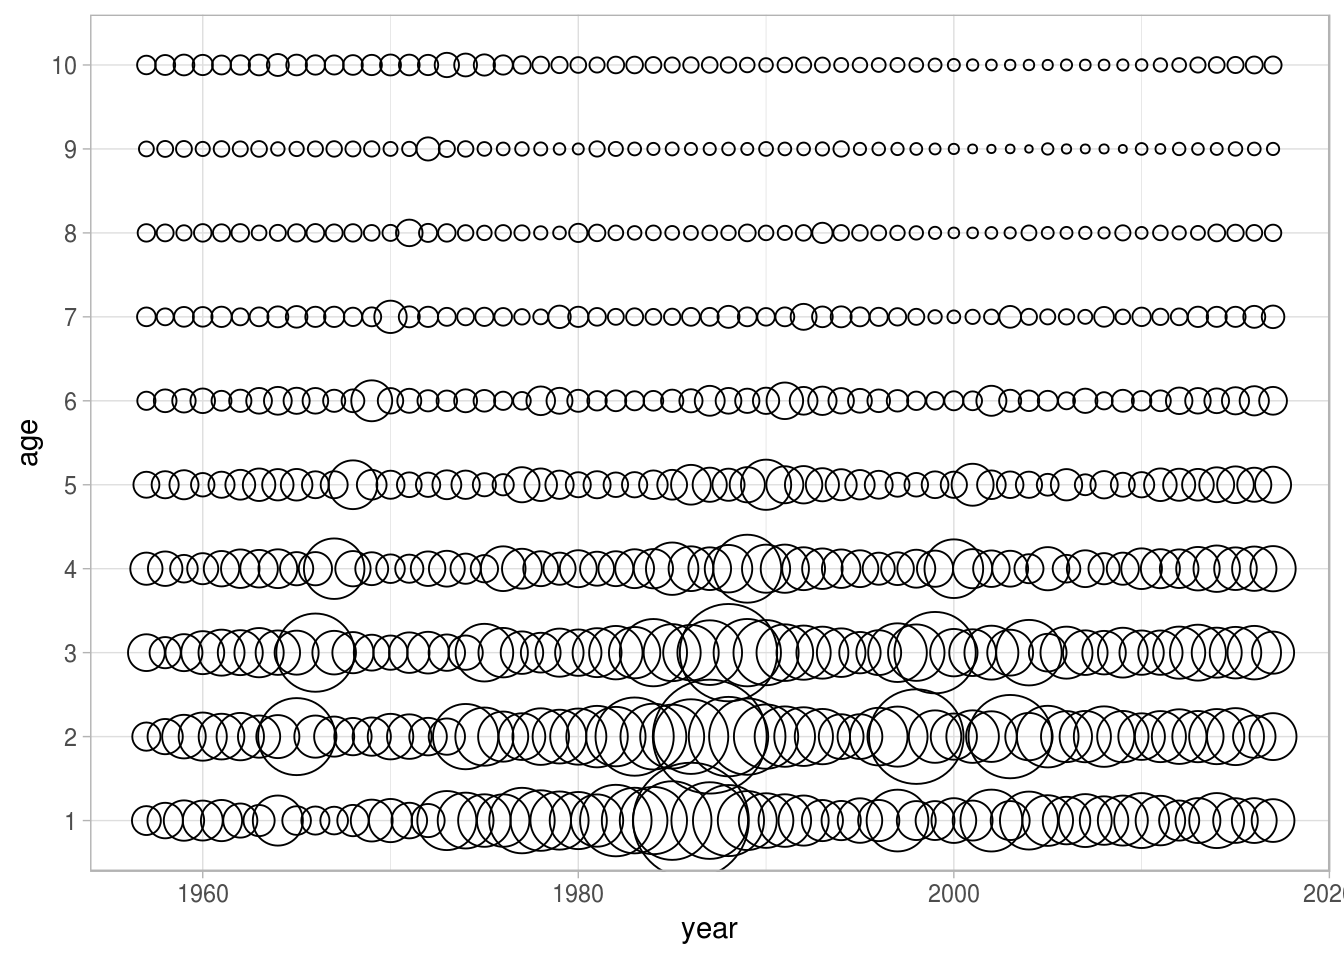
\includegraphics{docs/pdf/ggplotFL_plotting_FLR_objects_with_ggplot2_files/figure-latex/exbub-1} 

}

\caption{Bubble plot of catch by age in numbners for North Sea plaice.}\label{fig:exbub}
\end{figure}

where \emph{data} is used to size the bubbles in the call to
\emph{aes()}. This single line of code replaces the functionality
offered by the \emph{lattice}-based \texttt{bubbles()} method available
in \texttt{FLCore}.

\subsection{Example: Residual plots}\label{example-residual-plots}

Residuals plots can be built, for example, for the numbers-at-age in the
catch \texttt{FLQuant} by subtraction of the computed mean from the
data. Then bubble plots can be built in \texttt{ggplot}, with size
proportional to the residual and conditional colour coding for
positive/negative residuals.

\begin{Shaded}
\begin{Highlighting}[]
\NormalTok{dat <-}\StringTok{ }\KeywordTok{as.data.frame}\NormalTok{(}\KeywordTok{catch.n}\NormalTok{(ple4))}
\NormalTok{dat$resid <-}\StringTok{ }\NormalTok{dat$data -}\StringTok{ }\KeywordTok{mean}\NormalTok{(dat$data)}
\KeywordTok{ggplot}\NormalTok{(dat, }\KeywordTok{aes}\NormalTok{(year, }\KeywordTok{as.factor}\NormalTok{(age), }\DataTypeTok{size=}\NormalTok{resid)) +}
\StringTok{  }\KeywordTok{geom_point}\NormalTok{(}\DataTypeTok{shape=}\DecValTok{21}\NormalTok{, }\KeywordTok{aes}\NormalTok{(}\DataTypeTok{colour=}\KeywordTok{factor}\NormalTok{(}\KeywordTok{sign}\NormalTok{(resid)), }\DataTypeTok{fill=}\KeywordTok{factor}\NormalTok{(}\KeywordTok{sign}\NormalTok{(resid)))) +}
\StringTok{  }\KeywordTok{scale_size}\NormalTok{(}\DataTypeTok{range =} \KeywordTok{c}\NormalTok{(}\DecValTok{1}\NormalTok{, }\DecValTok{20}\NormalTok{)) +}
\StringTok{  }\KeywordTok{scale_colour_manual}\NormalTok{(}\DataTypeTok{values=}\KeywordTok{c}\NormalTok{(}\StringTok{"black"}\NormalTok{, }\StringTok{"white"}\NormalTok{)) +}
\StringTok{  }\KeywordTok{scale_fill_manual}\NormalTok{(}\DataTypeTok{values=}\KeywordTok{c}\NormalTok{(}\StringTok{"lightgray"}\NormalTok{, }\StringTok{"black"}\NormalTok{)) +}
\StringTok{  }\KeywordTok{ylab}\NormalTok{(}\StringTok{"age"}\NormalTok{)}
\end{Highlighting}
\end{Shaded}

\begin{figure}

{\centering 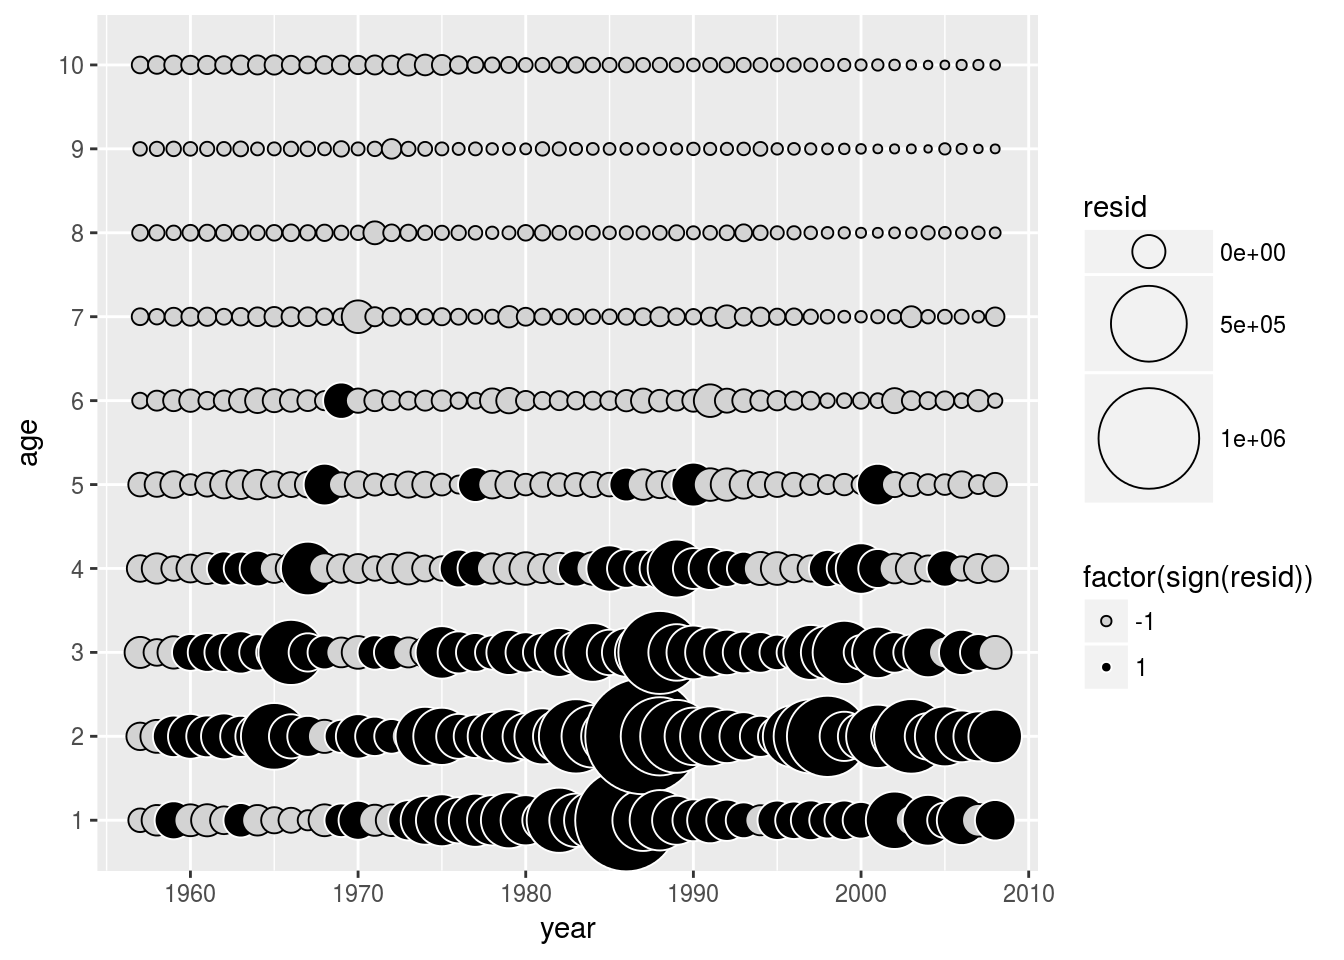
\includegraphics{docs/pdf/ggplotFL_plotting_FLR_objects_with_ggplot2_files/figure-latex/exres-1} 

}

\end{figure}

\section{References}\label{references}

Wilkinson, L. 1999. \emph{The Grammar of Graphics}, Springer.
\href{http://dx.doi.org/10.1007/978-3-642-21551-3_13}{doi
10.1007/978-3-642-21551-3\_13}

\section{More information}\label{more-information}

\begin{itemize}
\tightlist
\item
  You can submit bug reports, questions or suggestions on this tutorial
  at \url{https://github.com/flr/doc/issues}.
\item
  Or send a pull request to \url{https://github.com/flr/doc/}
\item
  For more information on the FLR Project for Quantitative Fisheries
  Science in R, visit the FLR webpage, \url{http://flr-project.org}.
\end{itemize}

\subsection{Software Versions}\label{software-versions}

\begin{itemize}
\tightlist
\item
  R version 3.5.1 (2018-07-02)
\item
  FLCore: 2.6.9.9007
\item
  ggplotFL: 2.6.4.9002
\item
  ggplot2: 3.0.0
\item
  \textbf{Compiled}: Wed Oct 3 11:47:24 2018
\end{itemize}

\subsection{License}\label{license}

This document is licensed under the
\href{https://creativecommons.org/licenses/by-sa/4.0}{Creative Commons
Attribution-ShareAlike 4.0 International} license.

\subsection{Author information}\label{author-information}

\textbf{Giacomo Chato Osio}, \textbf{Iago MOSQUEIRA}. European
Commission Joint Research Centre (JRC), Institute for the Protection and
Security of the Citizen (IPSC), Maritime Affairs Unit, Via E. Fermi
2749, 21027 Ispra VA, Italy. \url{https://ec.europa.eu/jrc/}

\textbf{Katell Hamon} Wageningen UR. Wageningen Economic Research.
Alexanderveld 5, The Hague, The Netherlands.

\end{document}
